\pagebreak
\chapter{Version Controll}
\setcounter{section}{0}

\section{GitHub Introduction}
\subsection{Befehle}
\begin{description}
	\item[my-slide Verzeichnis] % C:\Users\PaulJulitz\Documents\GitHub\github-slideshow %%% HP 
	\item[my-slide Verzeichnis] % C:\Users\Paul J\Documents\GitHub\github-slideshow %%% Dell 
	\item[git ls-files] Zeigt alle Dateien in einem Verzeichnis an.
	\item[copy con <file>] Dieser Befehl funktioniert unter Git bash. Die entsprechenden Datei wird in den aktiven Verzeichnis erstellt.
	\item[git status] Gib alle Änderungen eines Verzeichnises wieder.
	\item[git clone <URL.git>] Das URL mit .git wird in dem aktiven Verzeichnis geklont.
	\item[git branch <name>] Ein neuer Branch wird im lokalen Bereich erzeugt.
	\item[git checkout <local branch>] Ändert den aktiven lokalen Branch.
	\item[git push --set-upstream origin <Branch>] Der erzeugte Branch wird zum Remote Repository geladen.
	\item[git pull orign <Branch>] Ein Update (pull) eines spezifischen Branch wird gezogen.
	\item[git branch --all] Alle Branches lokal und remote werden angezeigt.
	\item[git branch -m <Name>] Der Name des Branches, welcher gerade aktiv ist, kann mit dem Befehl geändert werden.
	\item[git -add <file>] Bereitet Änderungen aus dem Working Bereich für den nächsten Commit vor.
	\item[git commit -m $"\dots "$] Mit jedem Commit wird ein Snapshot der Dateien gemacht. Diese werden unter \gls{VCS} abgespeichert. Eine Nachricht in notwendig.
	\item[git push] Alle Commit werden für den ausgewählten Branch gepusht.
	\item[git pull origin <Branch>] Aktualisiert den spezifischen Branch.
	\item[git merge <Branch>] Der Master Branch wird mit dem ausgewählten Branch vereinigt.
	\item[git branch -d <Branch>] Löscht den lokalen Branch, welcher schon mit master vereinigt ist.
	\item[git branch -D <Branch>] Löscht den lokalen Branch.
	\item[git push origin  --delete <Branch>] Löscht den remote Branch, solang er auf \gls{g_Git} Hub noch nicht $"$archiviert$"$ wurde, sonst kann der Branch nicht gefunden werden. 
	\item[git remote prune origin] Löscht leere Branch Hüllen.
\end{description}

\subsection{Unterschied zwischen git bash, cmd und gui}
\begin{description}
	\item[Git bash] Es handelt sich hier um eine UNIX \gls{g_Shell}. Dies bietet sich an, wenn Linux schon bekannt ist.
	\item[Git CMD] Es handelt sich hier um eine UNIX \gls{g_Shell}. Dies bietet sich an, wenn Windows bekannt ist.
	\item[Git GUI] Bietet die Funktionalität von git in einer grafische Oberfläche an.
\end{description} \cite{stackoverflow.Diff}

\subsubsection{Staging Area / Index / Cache}
Der Staging Bereich oder Index erlaubt inhaltlich verbundenen Dateien/ Änderungen an Dateien aus dem Working Bereich vorzuhalten und per \textbf{git add}. 
\begin{lstlisting}[style=CMD]
	C:\Users\Paul J\Documents\GitHub\github-slideshow> git status
	On branch dell_Branch
	Your branch is up to date with 'origin/dell_Branch'.
	
	Untracked files:
	(use "git add <file>..." to include in what will be committed)
	_ <@\textcolor{red}{posts/test-dell.md}@> - Copy.txt

	nothing added to commit but untracked files present (use "git add" to track)
\end{lstlisting}
Dateien, welche diesem Index zugeordnet wurden, werden per \textbf{git commit} mit einer Nachricht zum lokalen \gls{g_Git_Repository} übertragen. Die gesammelten Commits können per \textbf{git push} zum Remote Repository übertragen werden.
\begin{lstlisting}[style=CMD]
C:\Users\Paul J\Documents\GitHub\github-slideshow> git status
On branch dell_Branch
Your branch is ahead of 'origin/dell_Branch' by 1 commit.
(use "git push" to publish your local commits)

nothing to commit, working tree clean
\end{lstlisting}
\begin{figure}[H]
	\centering
	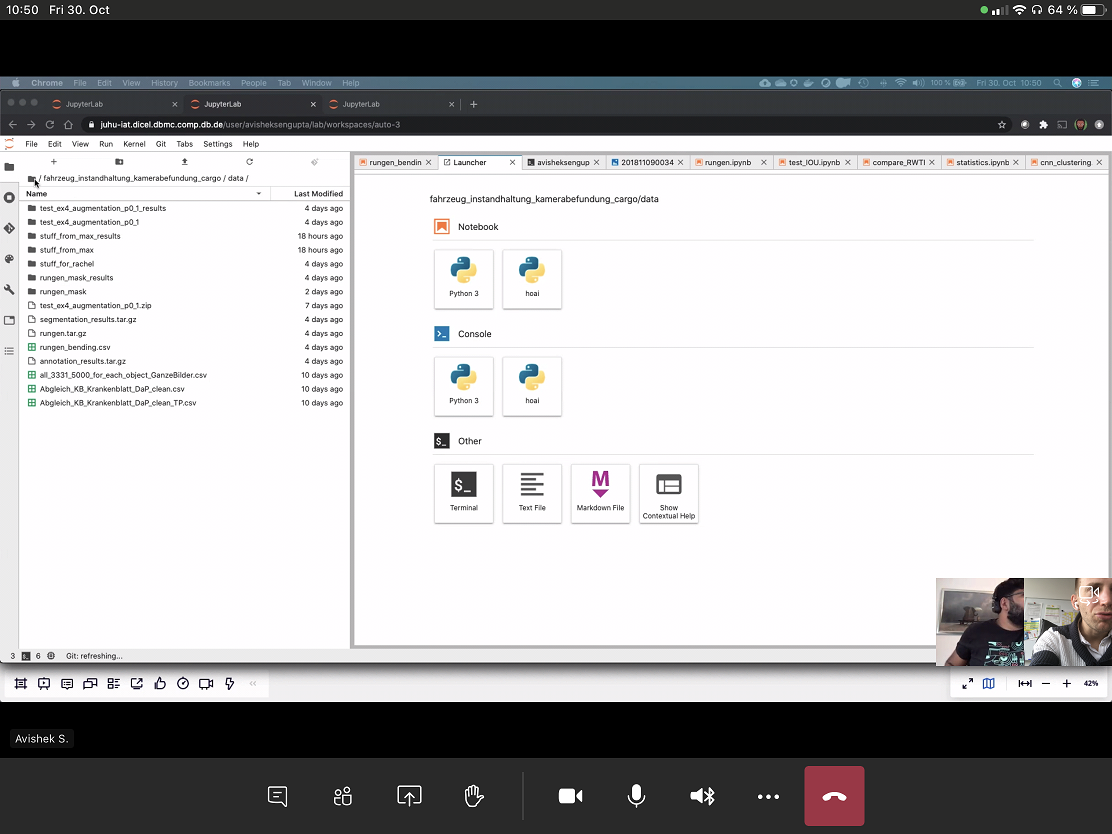
\includegraphics[width=0.7\linewidth]{attachment/chapter_6/Scc000}
\end{figure}

Eine Datei im \gls{g_Git} Ordner kann in zwei Kategorien untergliedert werden:
\begin{itemize}
	\item tracked und
	\item untracked.
\end{itemize}
In früheren \gls{g_Git} Versionen konnte eine ungetrackte Datei \gls{g_Git_Repository} zugeordnet werden ohne als \textit{staged} markiert zu werden, sodass sie Teil der \gls{VCS} wurde. Mit \textbf{git add <file>} wird diese Datei heute zum Staging Bereich zugeordnet und von \gls{g_Git} getrackt. Beim nächsten \textbf{git push} wird diese Datei ans Remote \gls{g_Git_Repository} gesendet.


Mit \gls{g_Git} GUI ist eine Übersicht gegeben, welche Dateien noch nicht im Stage Modus sind und welche schon. 
\begin{figure}[H]
	\centering
	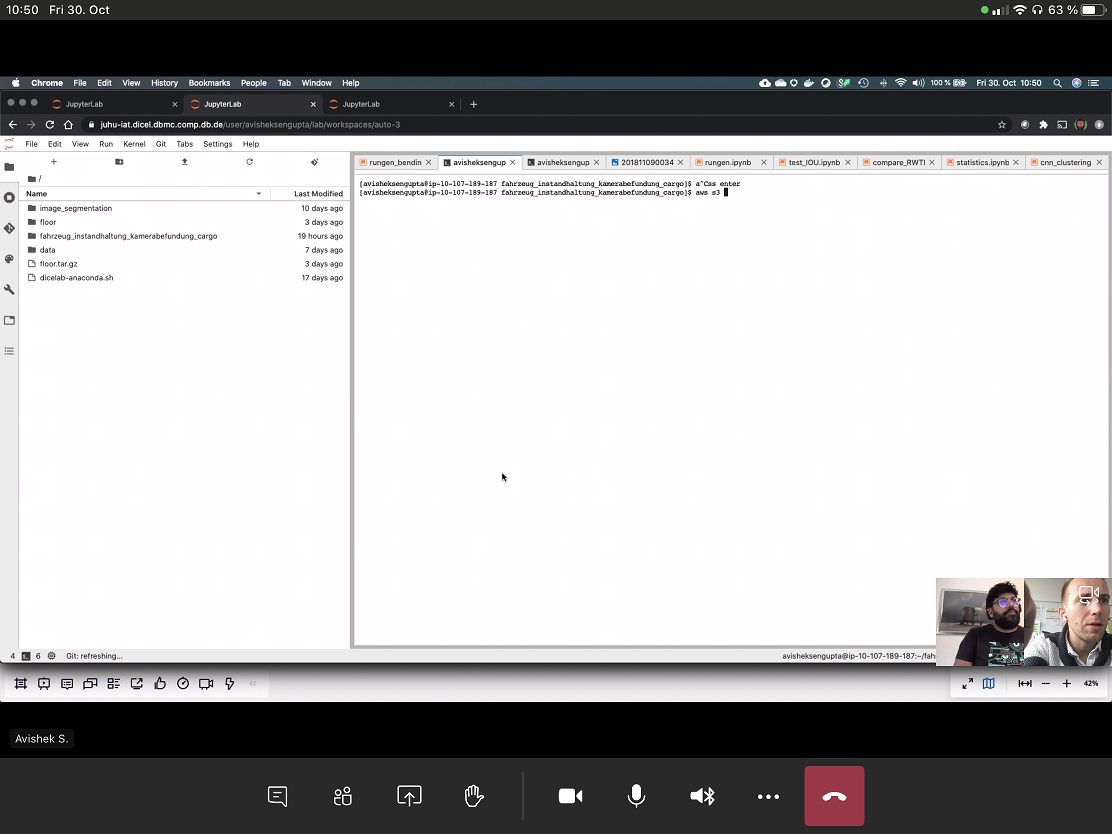
\includegraphics[width=0.7\linewidth]{attachment/chapter_6/Scc001}
\end{figure}
Die Commits werden pro Branch aufgeteilt.
\begin{figure}[H]
	\centering
	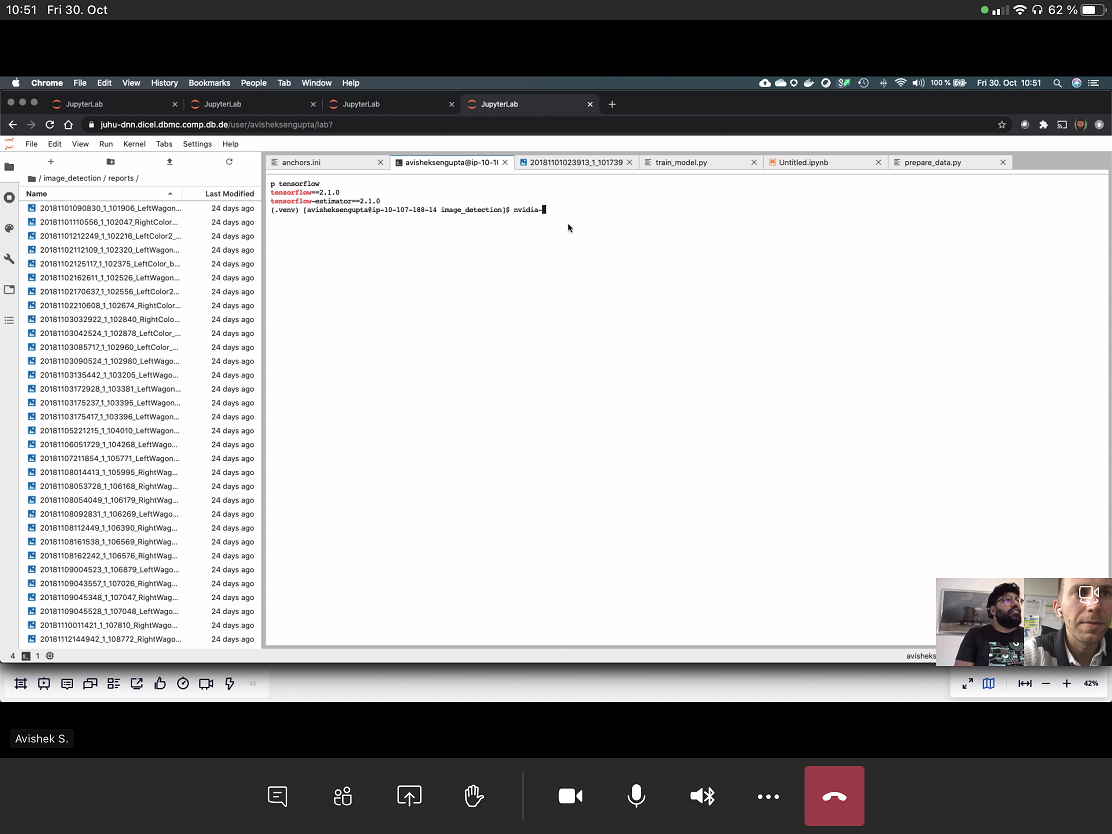
\includegraphics[width=0.7\linewidth]{attachment/chapter_6/Scc003}
\end{figure}
Zu jedem Schritt exisitert ein Befehl in \gls{g_Git_CMD}.
\begin{figure}[H]
	\centering
	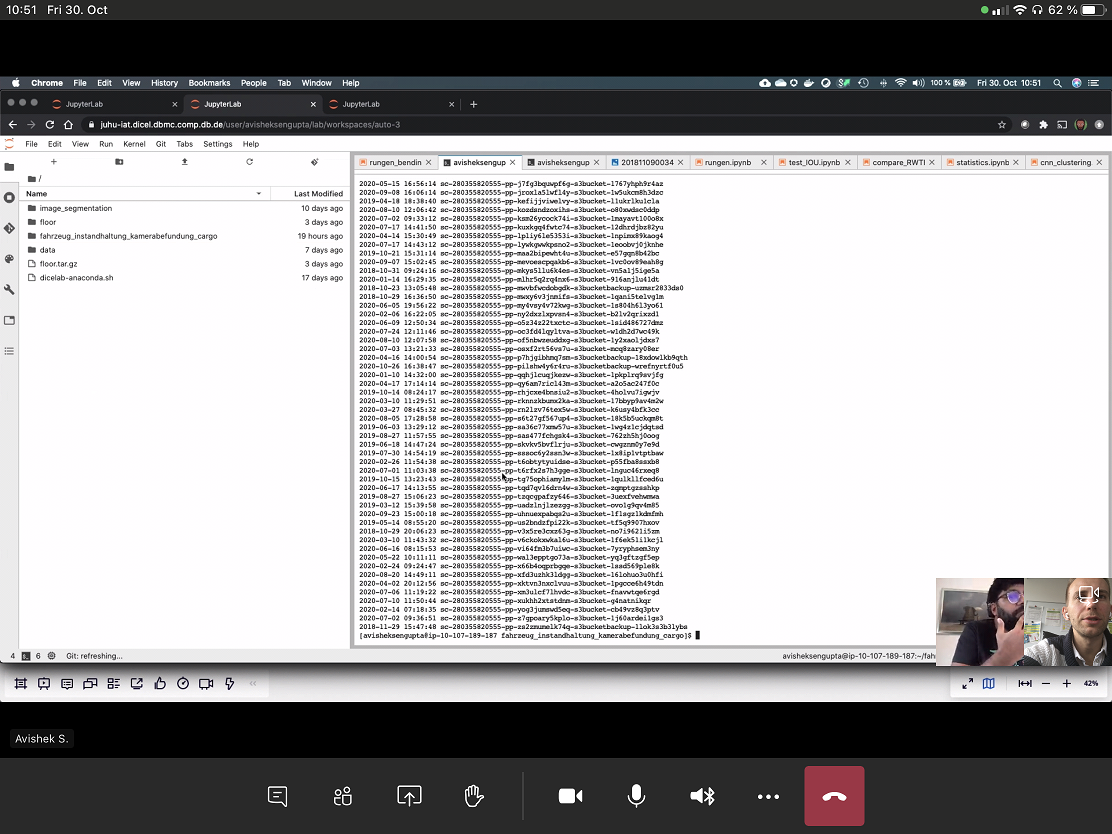
\includegraphics[width=0.7\linewidth]{attachment/chapter_6/Scc002}
\end{figure}

\subsubsection{Commiting}
Commits sind Snapshots/ Milestones des Projektes/ Ordners oder Dateien. Dies werden werden auf dem lokalen \gls{g_Git_Repository} abgespeichert. Commits können auch wieder gelöscht werden. Wenn alle Commits bereit sind, geteilt zu werden, können sie per \textbf{git push origin <Branch>} auf das remote \gls{g_Git_Repository} geladen werden. 
Über \gls{g_Git} Hub stehen die Veränderungen und die History bereit zur Bearbeitung.

\begin{figure}[H]
	\centering
	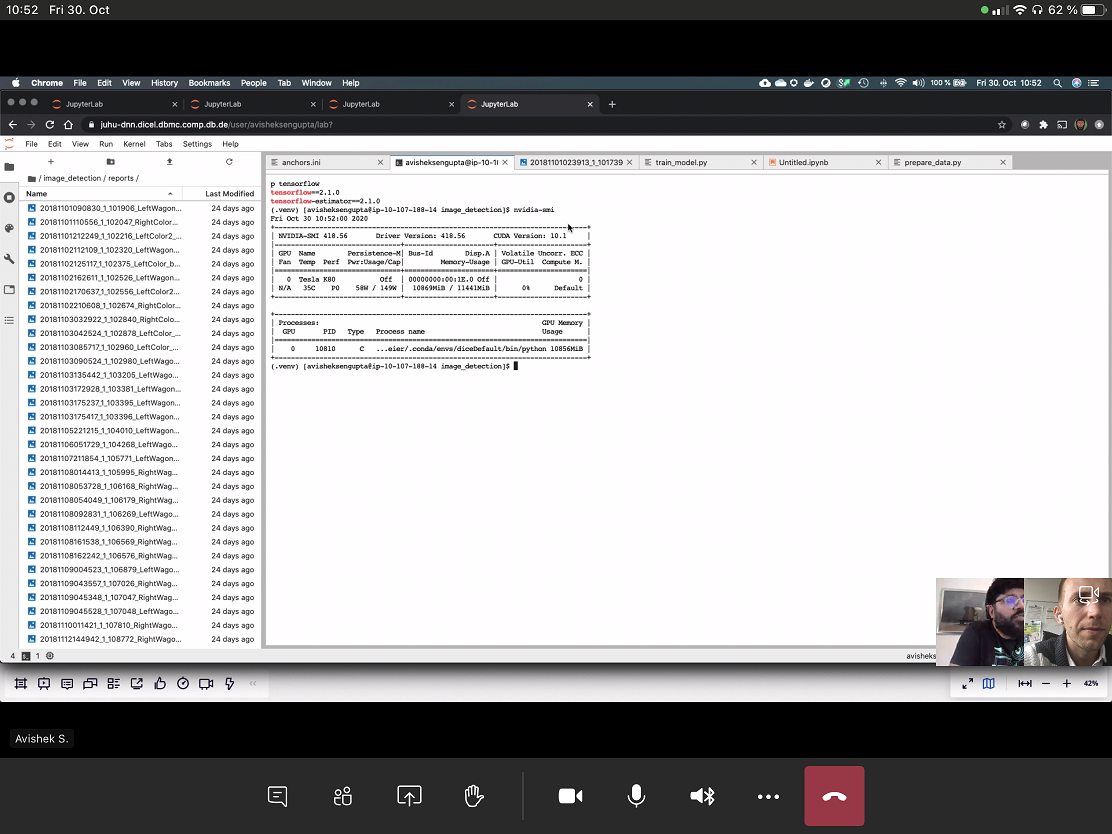
\includegraphics[width=0.7\linewidth]{attachment/chapter_6/Scc004}
	\caption{Richtig Auswahl des Branches $\&$ History anzeigen lassen.}
\end{figure}

\begin{figure}[H]
	\centering
	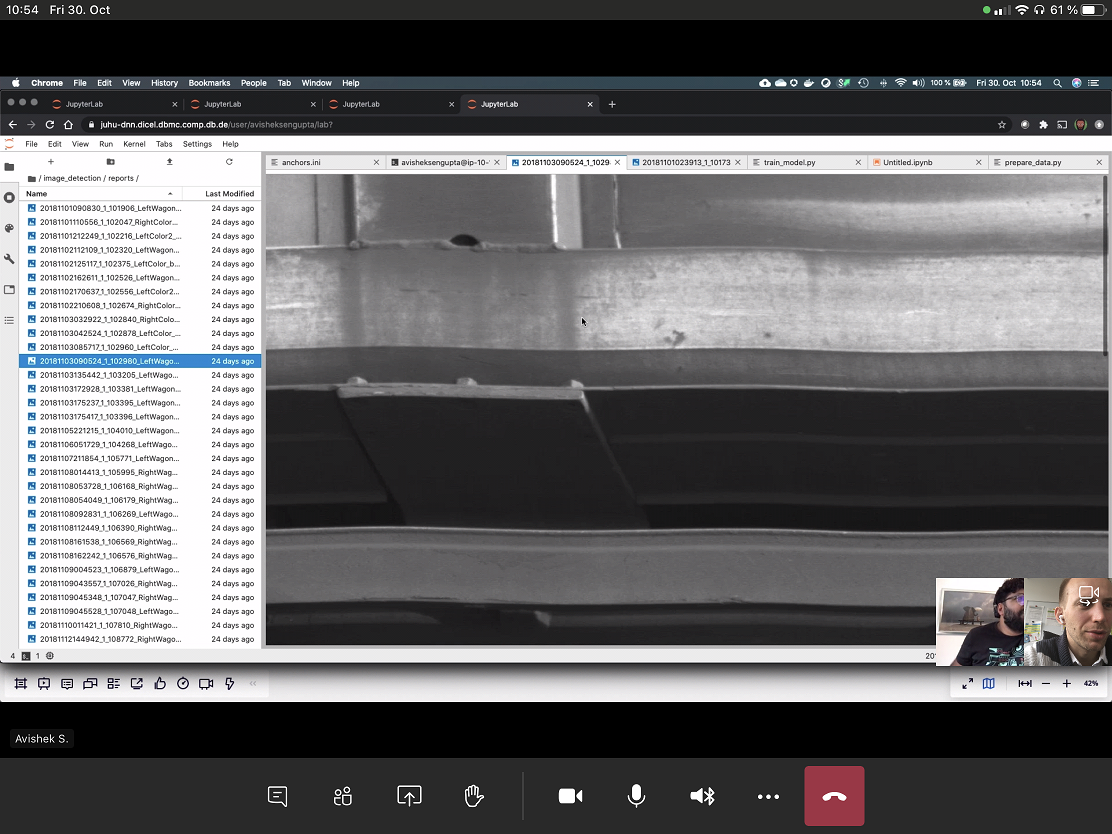
\includegraphics[width=0.7\linewidth]{attachment/chapter_6/Scc005}
	\caption{Zu jedem Milstone/ Linie besteht die Möglichkeit Kommentare anzubringen.}
\end{figure}

\subsection{Example: github-slideshow}
\subsubsection{Clone Respository and Create a Branch}
Ziel in diesem Abschnitt ist es, das 
Mit der Clone Anweisung wird das \gls{g_Git_Repository} auf den lokalen Server des Users gespielt. Die \gls{VCS} wird in Git hinterelegt und speichert die Änderungen an den Daten. Damit die Änderungen sich einfach einbinden lassen und von verschiedenen User erstellt werden, wird ein \textbf{Branch} erstellt. 

\begin{lstlisting}[style=CMD]
	/// Change directory to where the repository should be saved
	git cd C:\Users\PaulJulitz\Documents\GitHub
	/// Clone repository to local server (.../Username/NameRepository)
	git clone https://github.com/pauljulitz/github-slideshow.git /// 
	/// Navigate to the repository in your shell
	git cd C:\Users\PaulJulitz\Documents\GitHub\github-slideshow
	/// Create a new branch
	git branch my-slide
\end{lstlisting}

\subsubsection{Check all the branches of one repository}
In einem \gls{g_Git_Repository} können mehrere Branches erstellt werden. Welche für das gewissen \gls{g_Git_Repository} zugewissen sind, kann über \bl{branch --all} in einen \gls{g_Git_Repository} dargestellt werden.

\begin{lstlisting}[style=CMD]
	C:\Users\PaulJulitz>cd C:\Users\PaulJulitz\Documents\GitHub\github-slideshow
	
	C:\Users\PaulJulitz\Documents\GitHub\github-slideshow> git branch --all
	master
	*<@\textcolor{green}{my-slide}@>
	secoundBranch
	<@\textcolor{red}{remotes/origin/HEAD}@> -> origin/master
	<@\textcolor{red}{remotes/origin/master}@>
	<@\textcolor{red}{remotes/origin/my-slide}@>
	<@\textcolor{red}{remotes/origin/secoundBranch}@>
\end{lstlisting}

Der aktuelle Branch wird in \textcolor{green}{Grün} mit eine $*$ angezeigt.

\subsubsection{Chance branch name}
Mit dem Befehl \textbf{-m <new name>} kann der Name des lokalen, ausgewählten Branch geändert werden. Wenn jedoch der gleiche Name für einen Branch ausgewählt wurde, wird der Zusatz \textit{-lokal} angefügt.
\begin{lstlisting}[style=CMD]
	C:\Users\PaulJulitz\Documents\GitHub\github-slideshow> git branch -m newName
\end{lstlisting}
\subsubsection{Change aktiv branch}
Ein Branch kann mit \textbf{git checkout <local branch>} gewechselt werden.
\begin{lstlisting}[style=CMD]
C:\Users\PaulJulitz\Documents\GitHub\github-slideshow> git branch --all
master
* <@\textcolor{green}{my-slide}@>
secoundBranch
<@\textcolor{red}{remotes/origin/HEAD}@> -> origin/master
<@\textcolor{red}{remotes/origin/master}@>
<@\textcolor{red}{remotes/origin/my-slide}@>
<@\textcolor{red}{remotes/origin/secoundBranch}@>

C:\Users\PaulJulitz\Documents\GitHub\github-slideshow> git checkout secoundBranch
Switched to branch 'secoundBranch'
Your branch is up to date with 'origin/secoundBranch'.

C:\Users\PaulJulitz\Documents\GitHub\github-slideshow> git branch --all
master
my-slide
* <@\textcolor{green}{secoundBranch}@>
<@\textcolor{red}{remotes/origin/HEAD}@> -> origin/master
<@\textcolor{red}{remotes/origin/master}@>
<@\textcolor{red}{remotes/origin/my-slide}@>
<@\textcolor{red}{remotes/origin/secoundBranch}@>
\end{lstlisting}

\subsubsection{Push new local branch}
Mit \textbf{--set-upstream origin <branch>} wird der angesteuerte Branch hochgeladen.
\begin{lstlisting}[style=CMD]
	git push --set-upstream origin my-slide
\end{lstlisting}

\subsubsection{Check the status of a branch}
Der Befehl \textbf{git status} gibt an, 
\begin{itemize}
	\item welcher Branch aktuell aktiv ist, 
	\item ob es Änderungen im Origion Projekt gibt und
	\item welche Änderungen gepusht werden müssen.
\end{itemize}

\begin{lstlisting}[style=CMD]
	C:\Users\PaulJulitz\Documents\GitHub\github-slideshow> git status
	On branch secoundBranch
	Your branch is up to date with 'origin/secoundBranch'.
	
	nothing to commit, working tree clear
\end{lstlisting}

\subsubsection{Create a new file}
Unter Git CMD wird der Befehl \textbf{copy con} nicht ausgeführt. Der Befehl \textbf{ls} ebenso nicht. Mit  

\subsubsection{Update Branch}
Mit dem Befehl \textbf{git pull origin <branch>} wird der spezifische Branch aktualisiert.
\begin{lstlisting}[style=CMD]
C:\Users\PaulJulitz\Documents\GitHub\github-slideshow> git pull origin my-slide
remote: Enumerating objects: 10, done.
remote: Counting objects: 100% (10/10), done.
remote: Compressing objects: 100% (7/7), done.
remote: Total 8 (delta 3), reused 0 (delta 0), pack-reused 0
Unpacking objects: 100% (8/8), 1.46 KiB | 14.00 KiB/s, done.
From https://github.com/pauljulitz/github-slideshow
* branch            my-slide   -> FETCH_HEAD
d64d186..e0c65fb  my-slide   -> origin/my-slide
Updating d64d186..e0c65fb
Fast-forward
_posts/0000-01-02-PaulJulitz.md | 6 ++++++
1 file changed, 6 insertions(+)
create mode 100644 _posts/0000-01-02-PaulJulitz.md

C:\Users\PaulJulitz\Documents\GitHub\github-slideshow> git status
On branch my-slide
Your branch is up to date with 'origin/my-slide'.

nothing to commit, working tree clean
\end{lstlisting}
\subsubsection{Pull Request}
Die kann über Github selbst erfolgen: 

\begin{figure}[H]
	\centering
	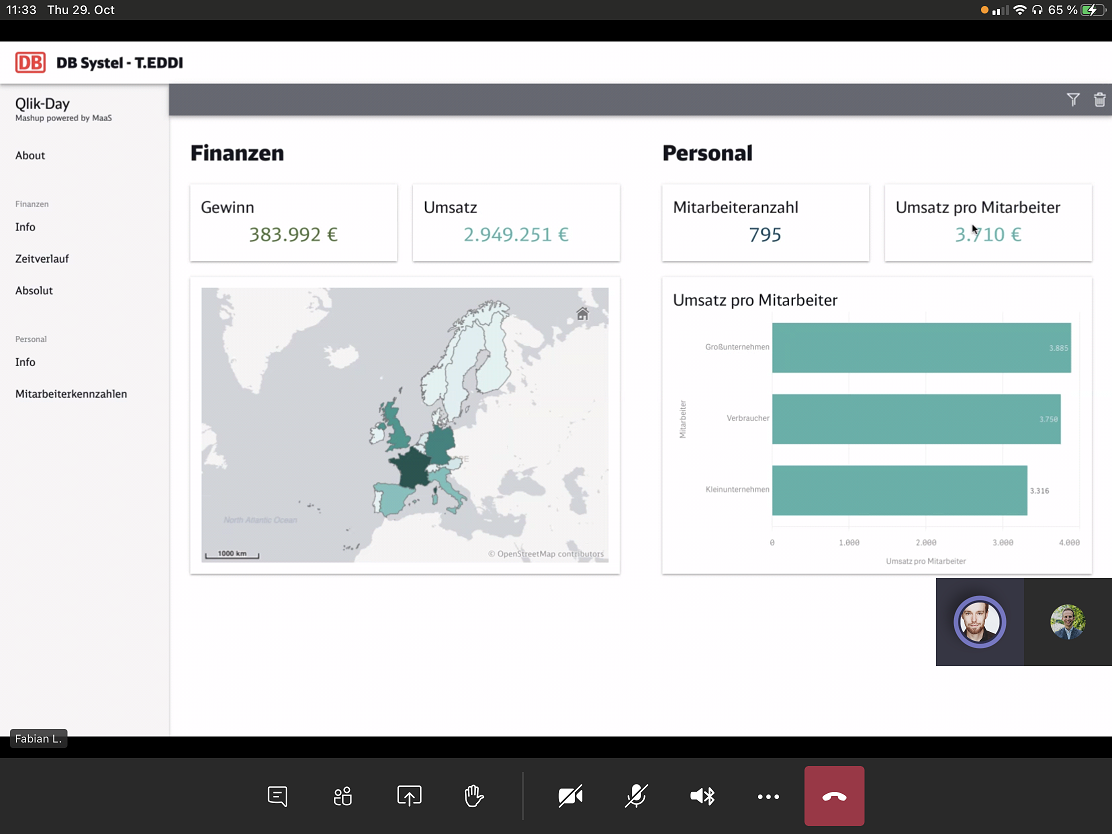
\includegraphics[width=0.7\linewidth]{attachment/chapter_6/Scc006}
\end{figure}

Oder über \gls{CMD} sind die folgenden Schritte notwendig.
Der Master Branch wird aktiviert. 
\begin{lstlisting}[style=CMD]
	C:\Users\PaulJulitz\Documents\GitHub\github-slideshow> git checkout master
\end{lstlisting}
Der benötigte Branch wird über \textbf{git merge} vereinigt.
\begin{lstlisting}[style=CMD]
	C:\Users\PaulJulitz\Documents\GitHub\github-slideshow> git merge my-slide
\end{lstlisting}
Dieser muss jetzt gepusht werden.
\begin{lstlisting}[style=CMD]
	C:\Users\PaulJulitz\Documents\GitHub\github-slideshow> git push
\end{lstlisting}
Der alte Branch kann jetzt gelöscht werden.
\begin{lstlisting}[style=CMD]
	C:\Users\PaulJulitz\Documents\GitHub\github-slideshow> git branch -d my-slide
\end{lstlisting}

\subsubsection{Delete local branch}
Wenn die Veränderungen überprüft wurden und der Branch vereingt wurde, wird das Prinzip verfolgt, den Branch zu löschen. 
Wenn dies über die \gls{g_Git} Hub Plattform passt, so bleibt eine $"$Ablage$"$ weiter bestehen.
\begin{figure}[H]
	\centering
	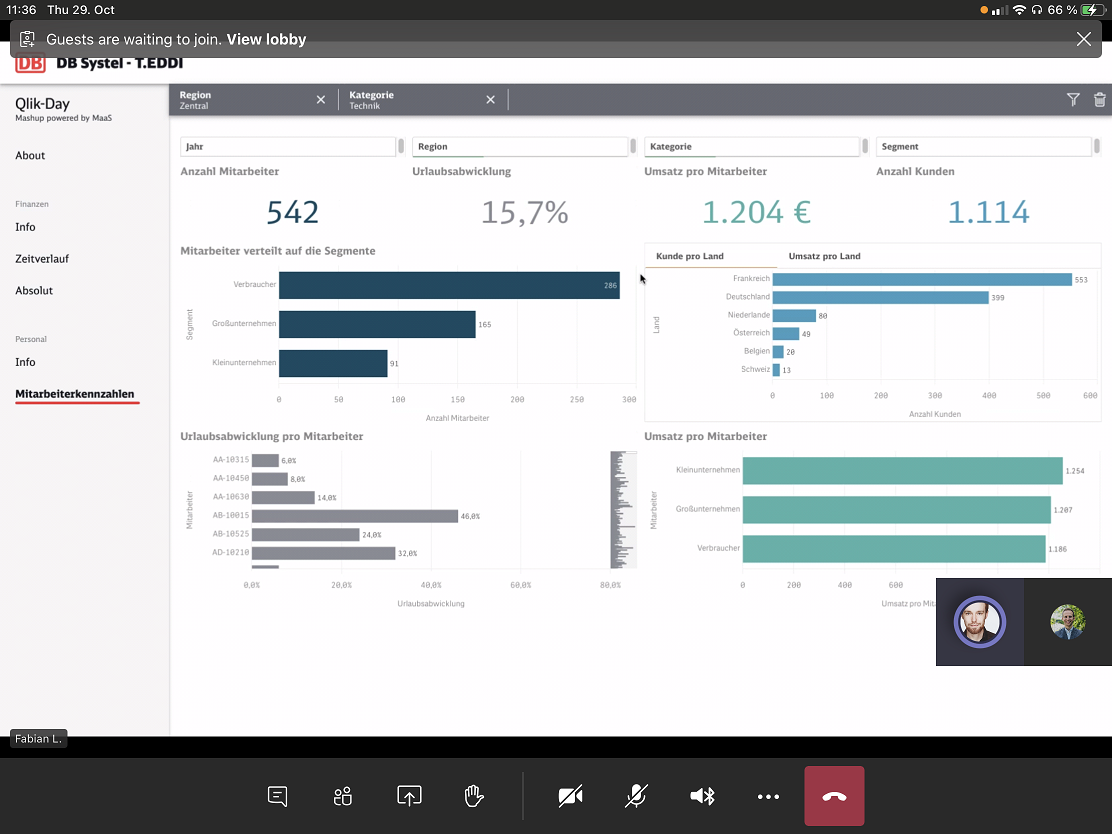
\includegraphics[width=0.7\linewidth]{attachment/chapter_6/Scc007}
\end{figure}
\begin{lstlisting}[style=CMD]
	C:\Users\Paul J\Documents\GitHub\github-slideshow>git push origin --delete dell_Branch
	error: unable to delete 'dell_Branch': remote ref does not exist
	<@\textcolor{red}{error: failed to push some refs to 'https://github.com/PaulJulitz/github-slideshow.git'}@>
\end{lstlisting}
Wenn dies nicht getan wurde oder der Branch wieder zurückrückgesetz wurde, wird er remote Branch gelöscht, durch: 

\begin{lstlisting}[style=CMD]
C:\Users\Paul J\Documents\GitHub\github-slideshow>git branch --all
* dell_Branch
master
remotes/origin/HEAD -> origin/master
<@\textcolor{red}{remotes/origin/dell$\_$ Branch}@>
<@\textcolor{red}{remotes/origin/dell$\_$Branch$\_$II}@>
remotes/origin/master
remotes/origin/my-slide
remotes/origin/secoundBranch

C:\Users\Paul J\Documents\GitHub\github-slideshow>git pull
Already up to date.

C:\Users\Paul J\Documents\GitHub\github-slideshow>git push origin --delete dell_Branch_II
To https://github.com/PaulJulitz/github-slideshow.git
- [deleted]         dell_Branch_II

C:\Users\Paul J\Documents\GitHub\github-slideshow>git push origin --delete dell_Branch
To https://github.com/PaulJulitz/github-slideshow.git
- [deleted]         dell_Branch

C:\Users\Paul J\Documents\GitHub\github-slideshow>git branch --all
* dell_Branch
master
remotes/origin/HEAD -> origin/master
remotes/origin/master
remotes/origin/my-slide
remotes/origin/secoundBranch
\end{lstlisting}

\subsubsection{Delete remote branch}
Der Befehl ist \textbf{git push origin --delete origin/<branch>}. Dieser ist an ein Pull Request welcher den Branch im remote \gls{g_Git_Repository} löscht. Wenn dieser Branch nicht mehr existiert, kommt ein Fehler zurück.

\subsubsection{Prune deletet remote branches}
Der Befehl \textbf{git remote prune origin} löscht alle Hüllen eines Branches.

\subsection{Designing your Github Page}
Formatierung einer .md Datei. Das README.md wir als Startseite unter der Auflistung der Daten angezeigt. Dies zu Formatieren kann helfen, eine Einführung in das \gls{g_Git_Repository} zu geben.
\begin{itemize}
	\item Ein Hashtag oder mehrere Hastagss geben die Größe der Überschrift an. 
	\item Bilder aus dem Web werden per ![profile-image](https://apod.nasa.gov/...%apod/image/1907/SpotlessSunIss_Colacurcio_2048.jpg)
	eingefügt.
	\item Wenn nur ein Bildlink eingefügt werden soll, muss das \textbf{!} vor dem Platzhaltern $[\dots]$. 
	\item Die Logik von Whatsapp ist auch hier Teilweise bei .md Formartierung anzuwenden (Kursiv, Fett, List).
\end{itemize} 

\section{GitLab Introduction}
Dieser Kurs ist ein Einsteigerkurs. Im Weiteren werden nur die wichtigsten oder neuesten Erkenntnisse notiert.

\subsection{Blame}

Mit der Blame-Funktion kann der Versionsverlauf einer bestimmten Datei nachgeschlagen werden.

\begin{figure}[H]
	\centering
	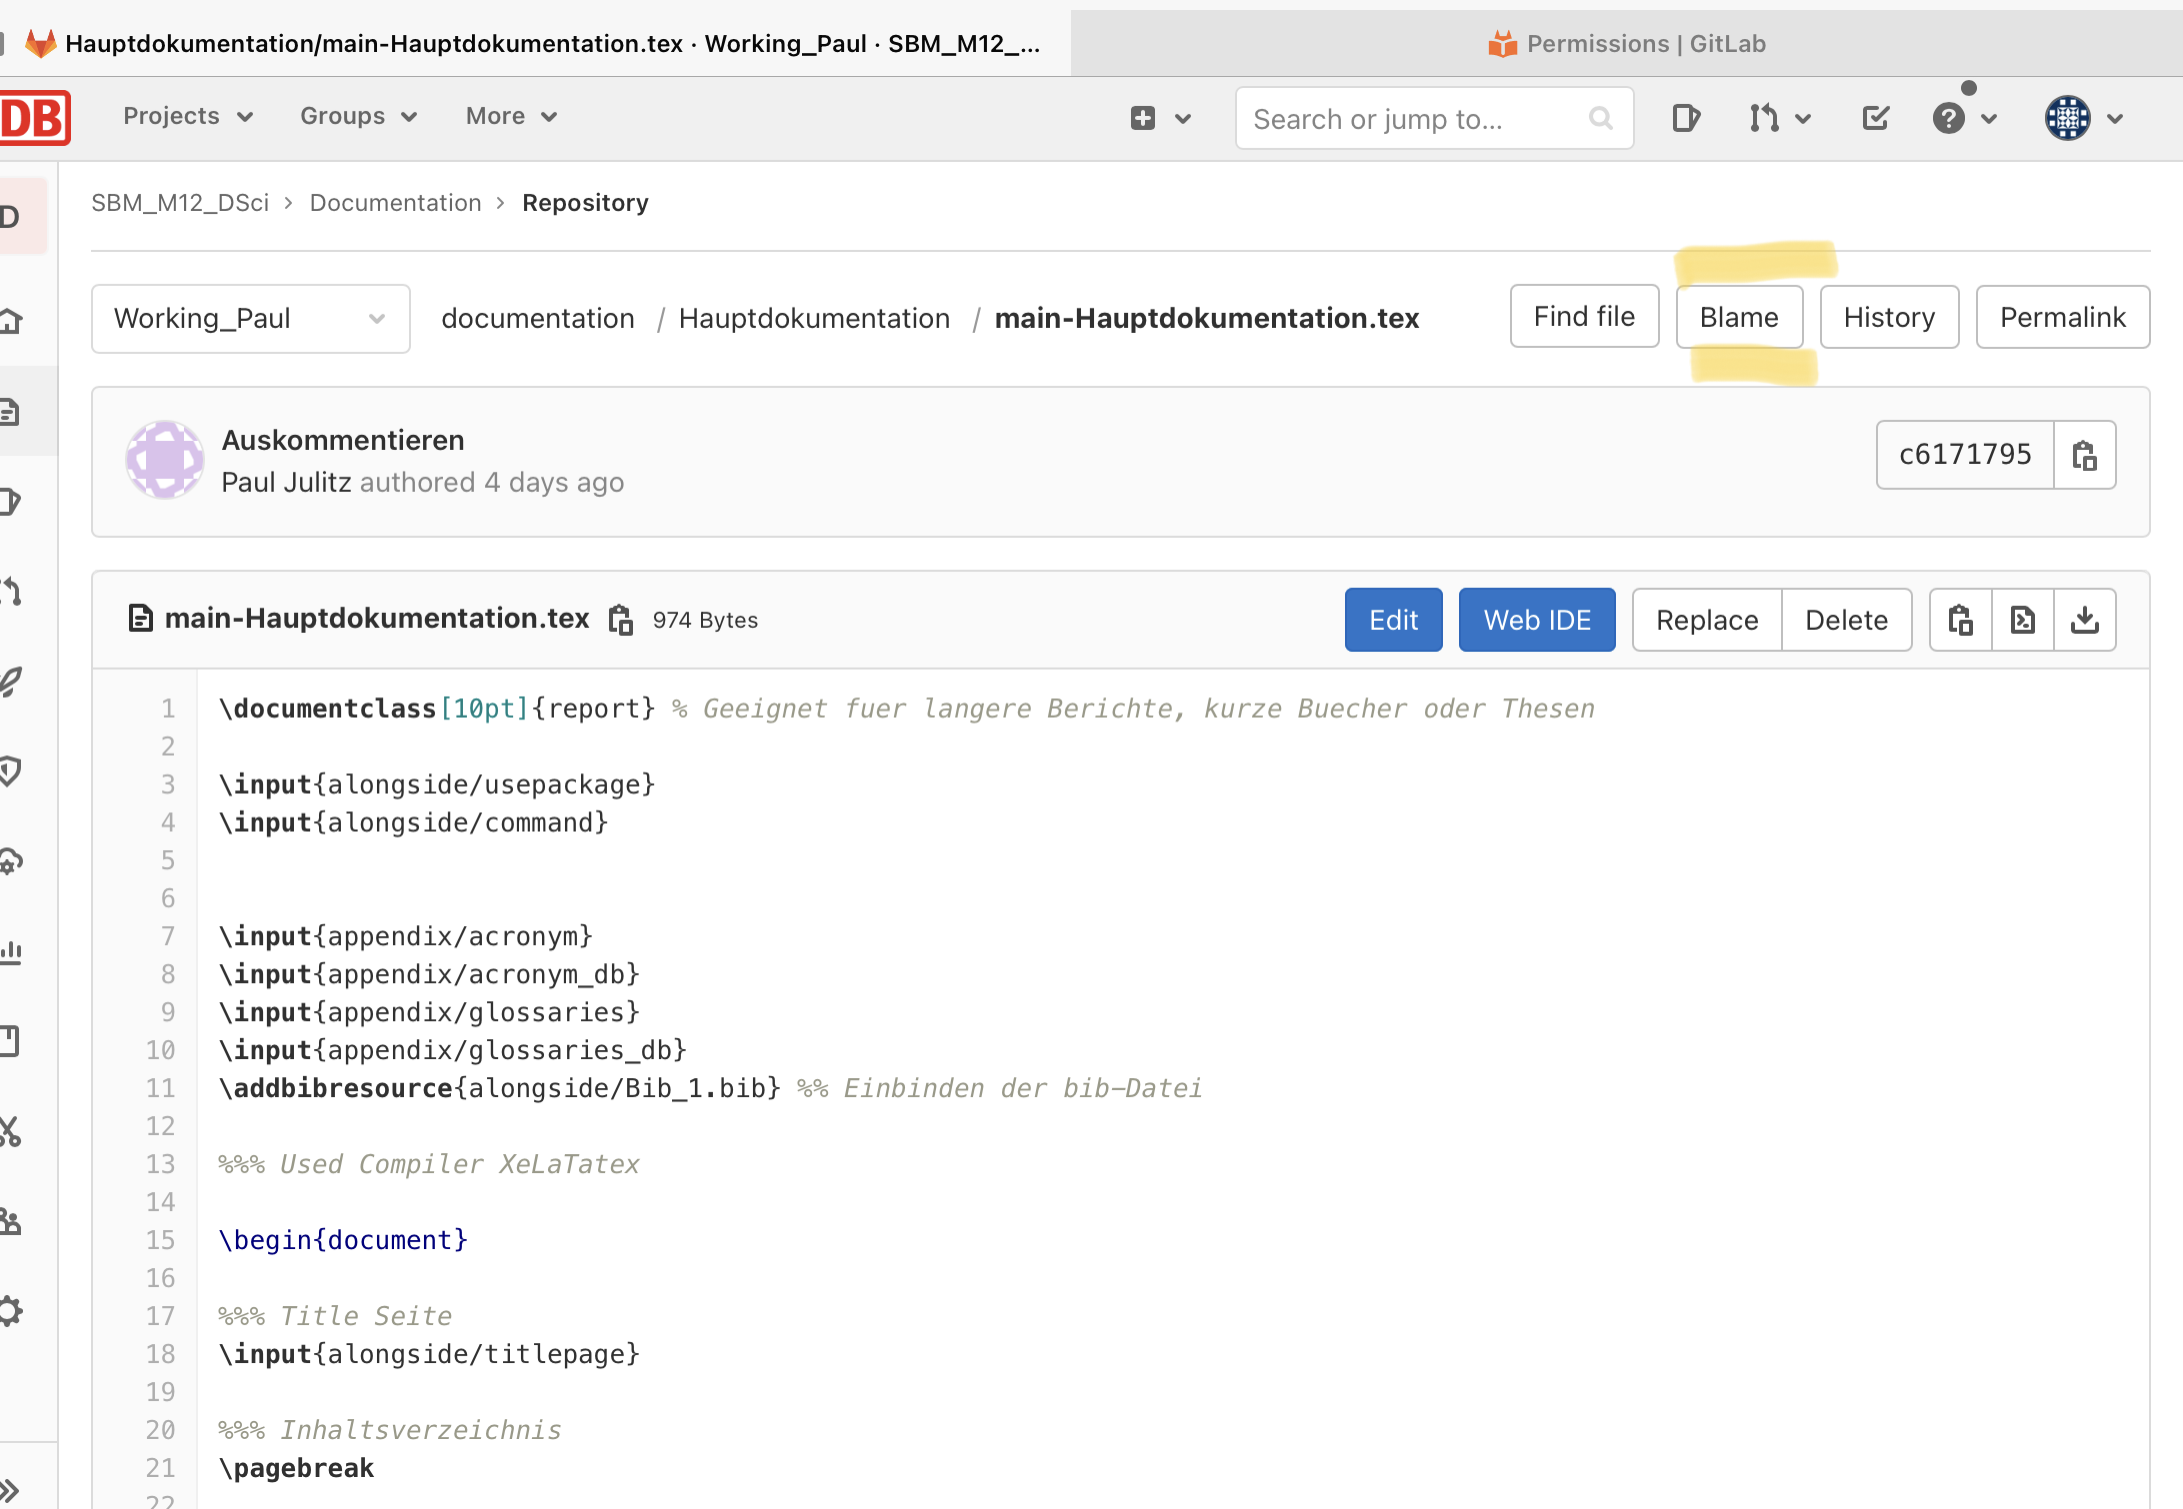
\includegraphics[width=0.7\linewidth]{attachment/chapter_5/Scc009}
\end{figure}

Dabei werden die Commits und die Veränderung direkt nebeneinander angezeigt.

\begin{figure}[H]
	\centering
	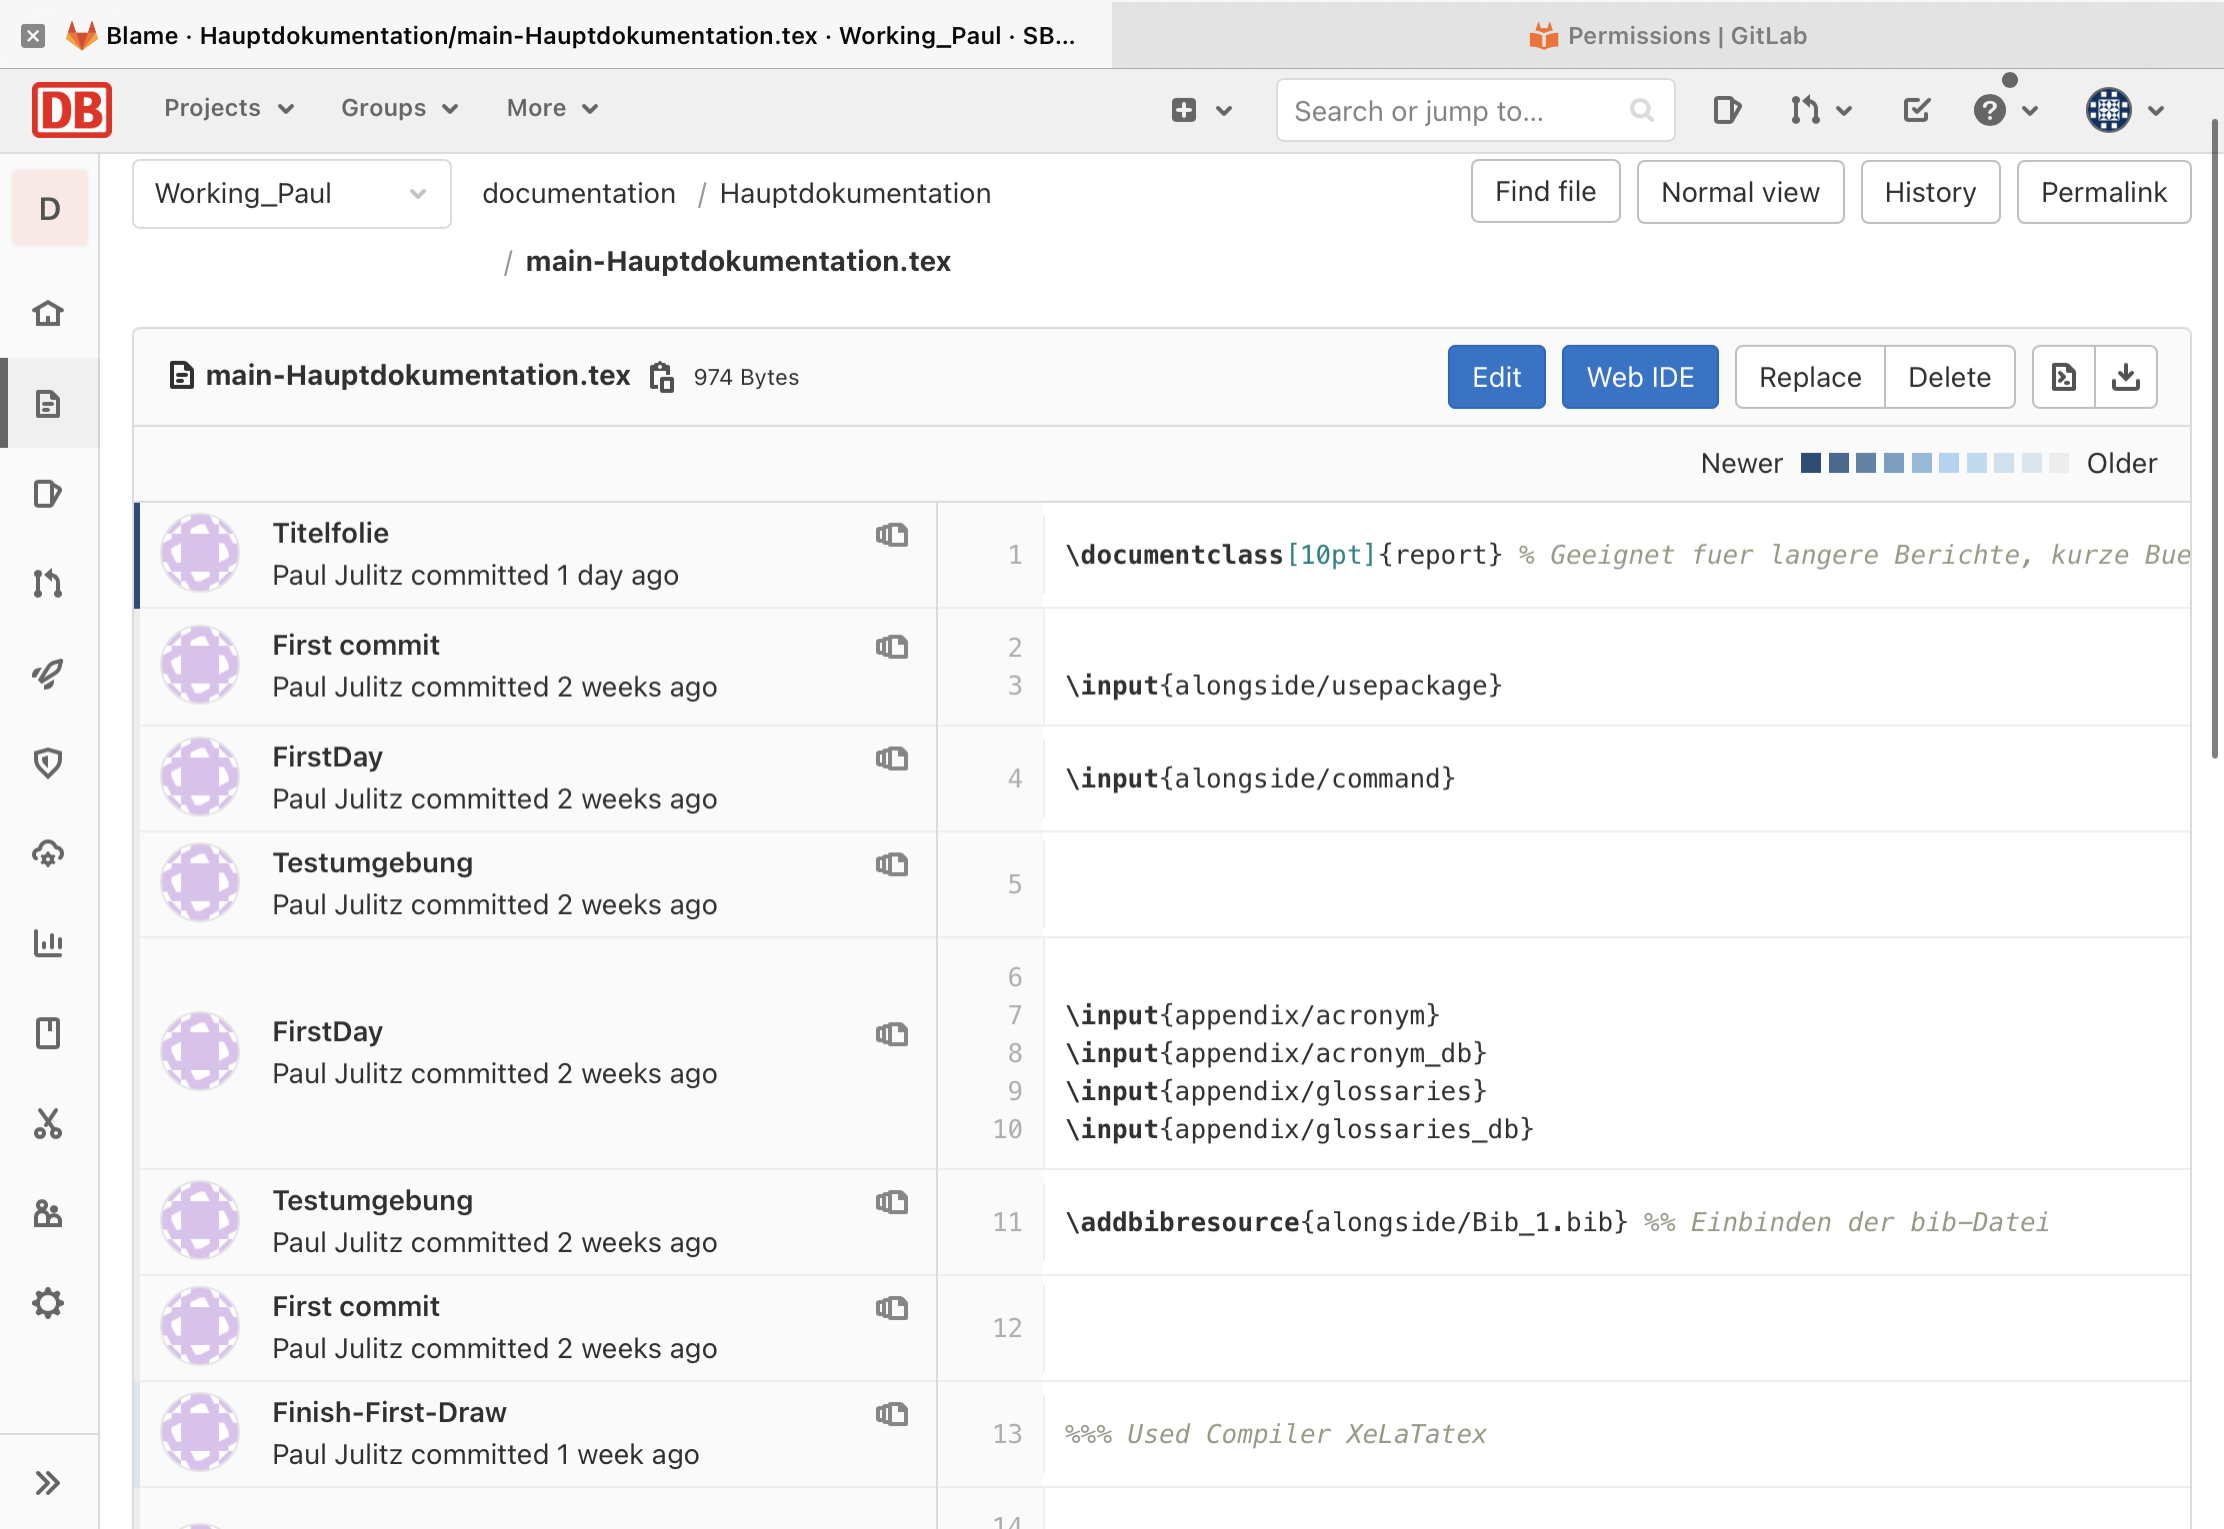
\includegraphics[width=0.7\linewidth]{attachment/chapter_5/Scc008}
\end{figure}

Dies unterscheide die History Funtkion, welche nur die Commit History anzeigt.

\begin{figure}[H]
	\centering
	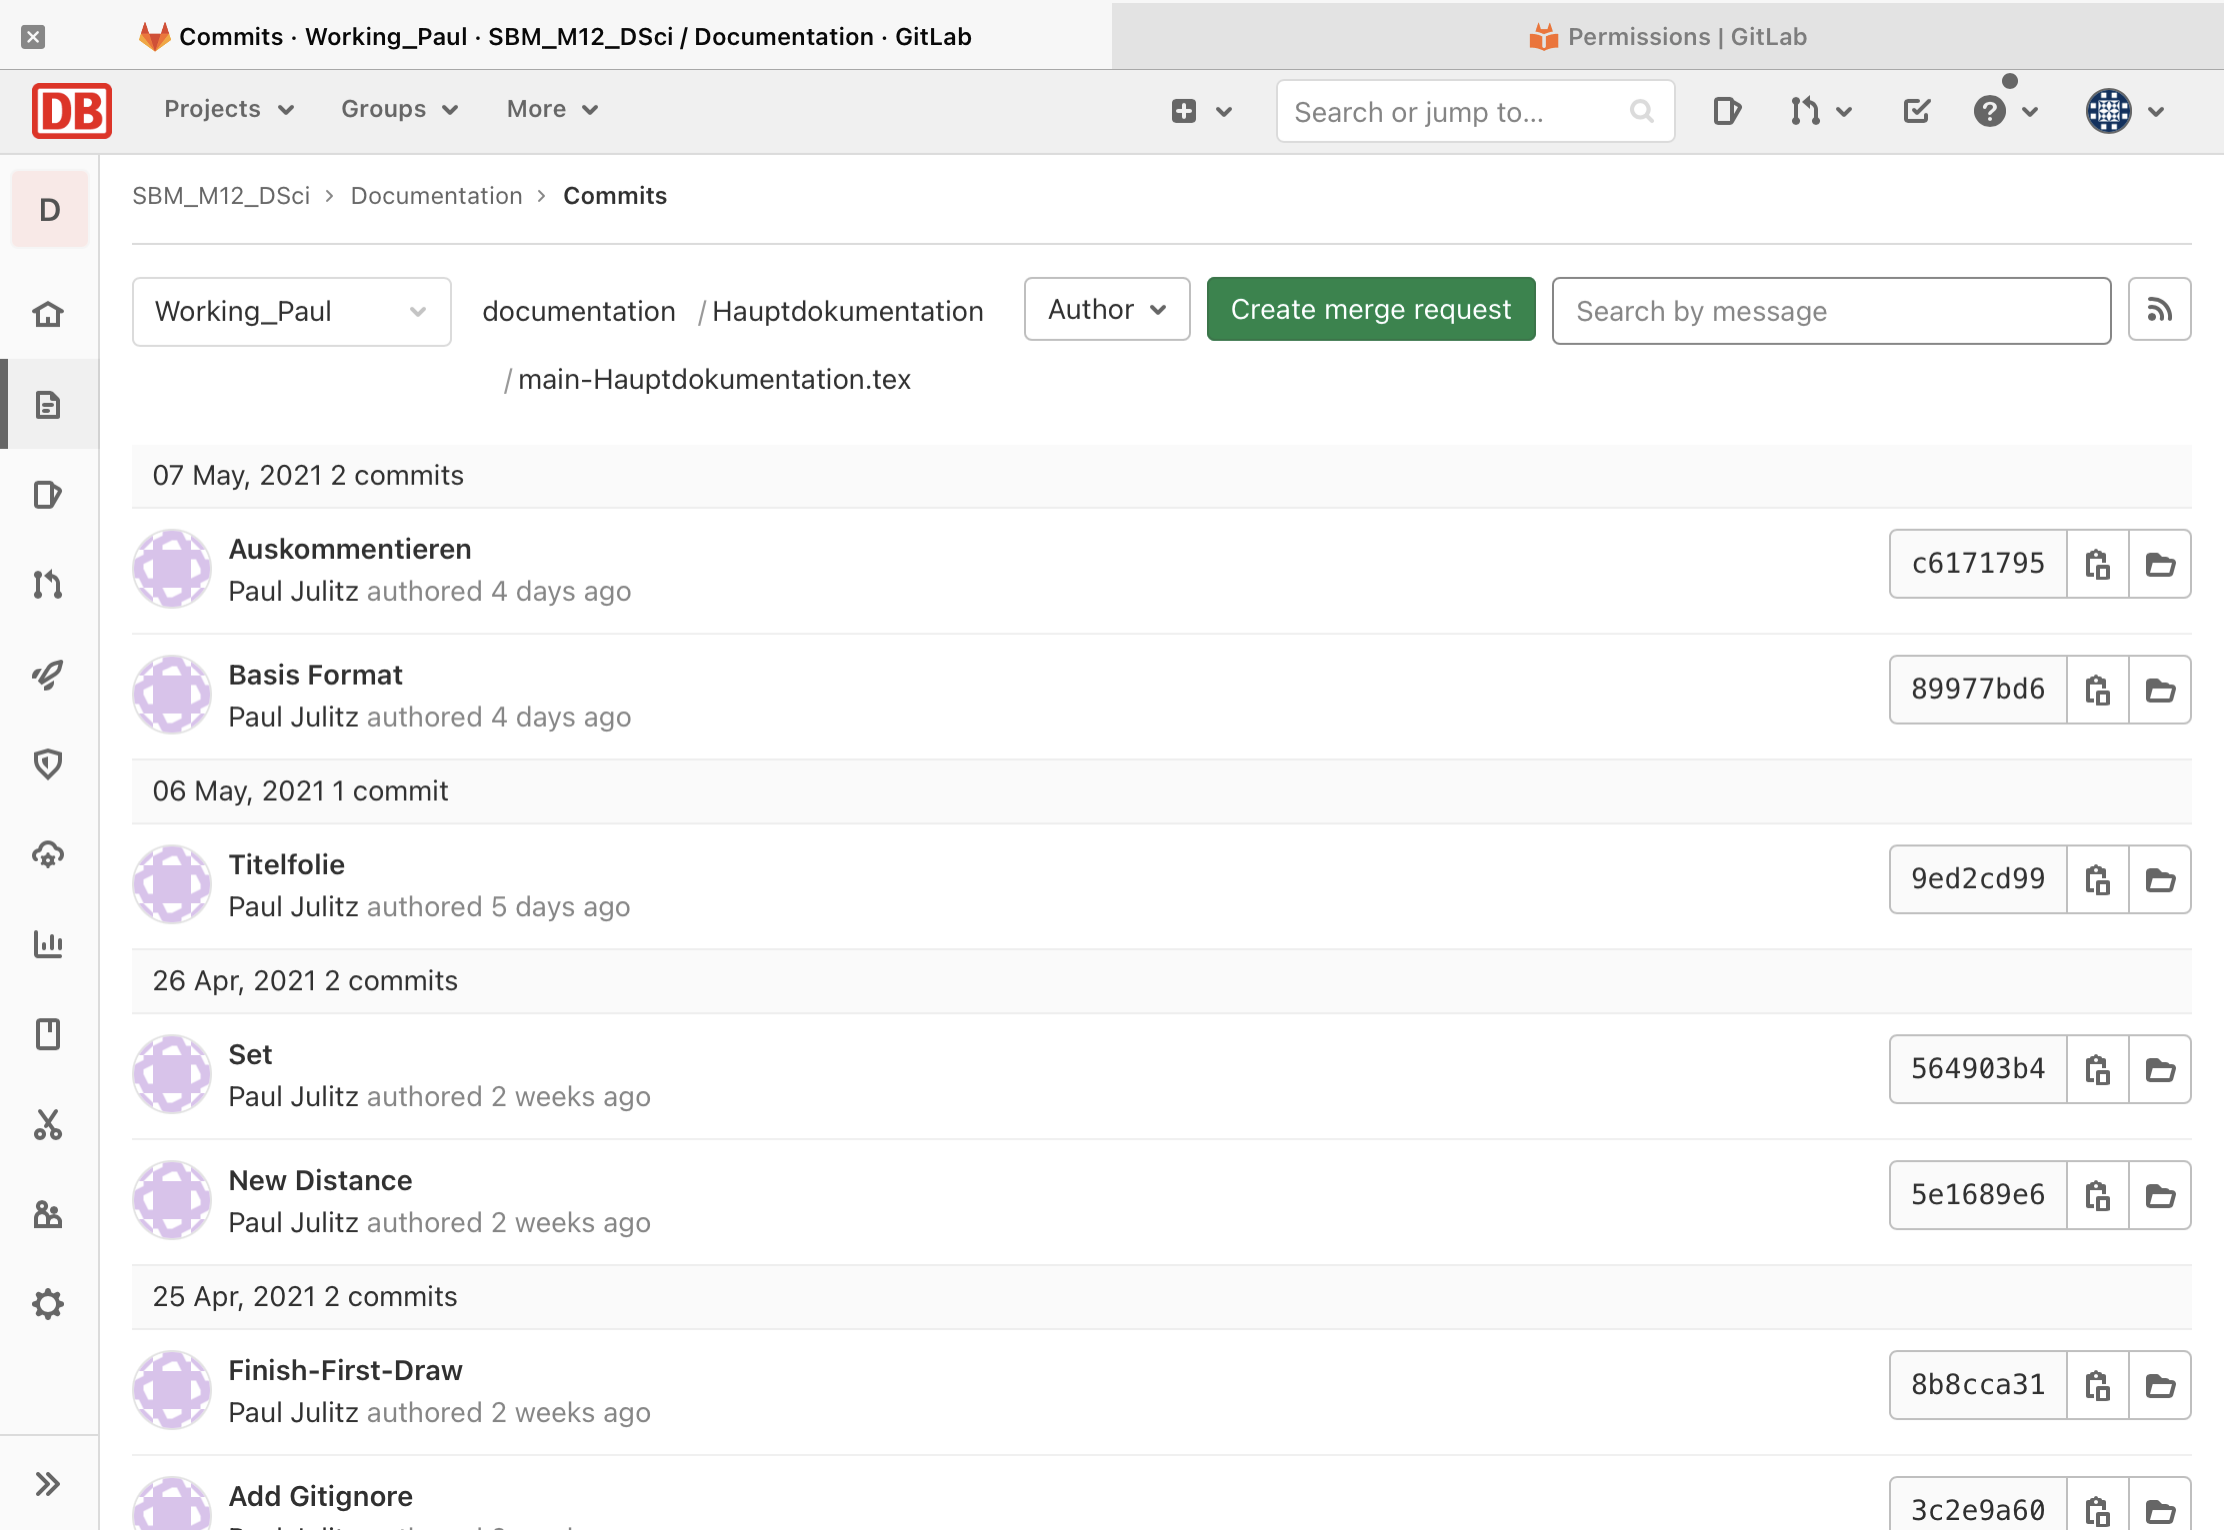
\includegraphics[width=0.7\linewidth]{attachment/chapter_5/Scc010}
\end{figure}

\subsection{Groups and Subgroups}
Unter Gruppen können auch Subgruppen erstellt werden. Diese dienen einen klarern Überblick zu schaffen.

\begin{figure}[H]
	\centering
	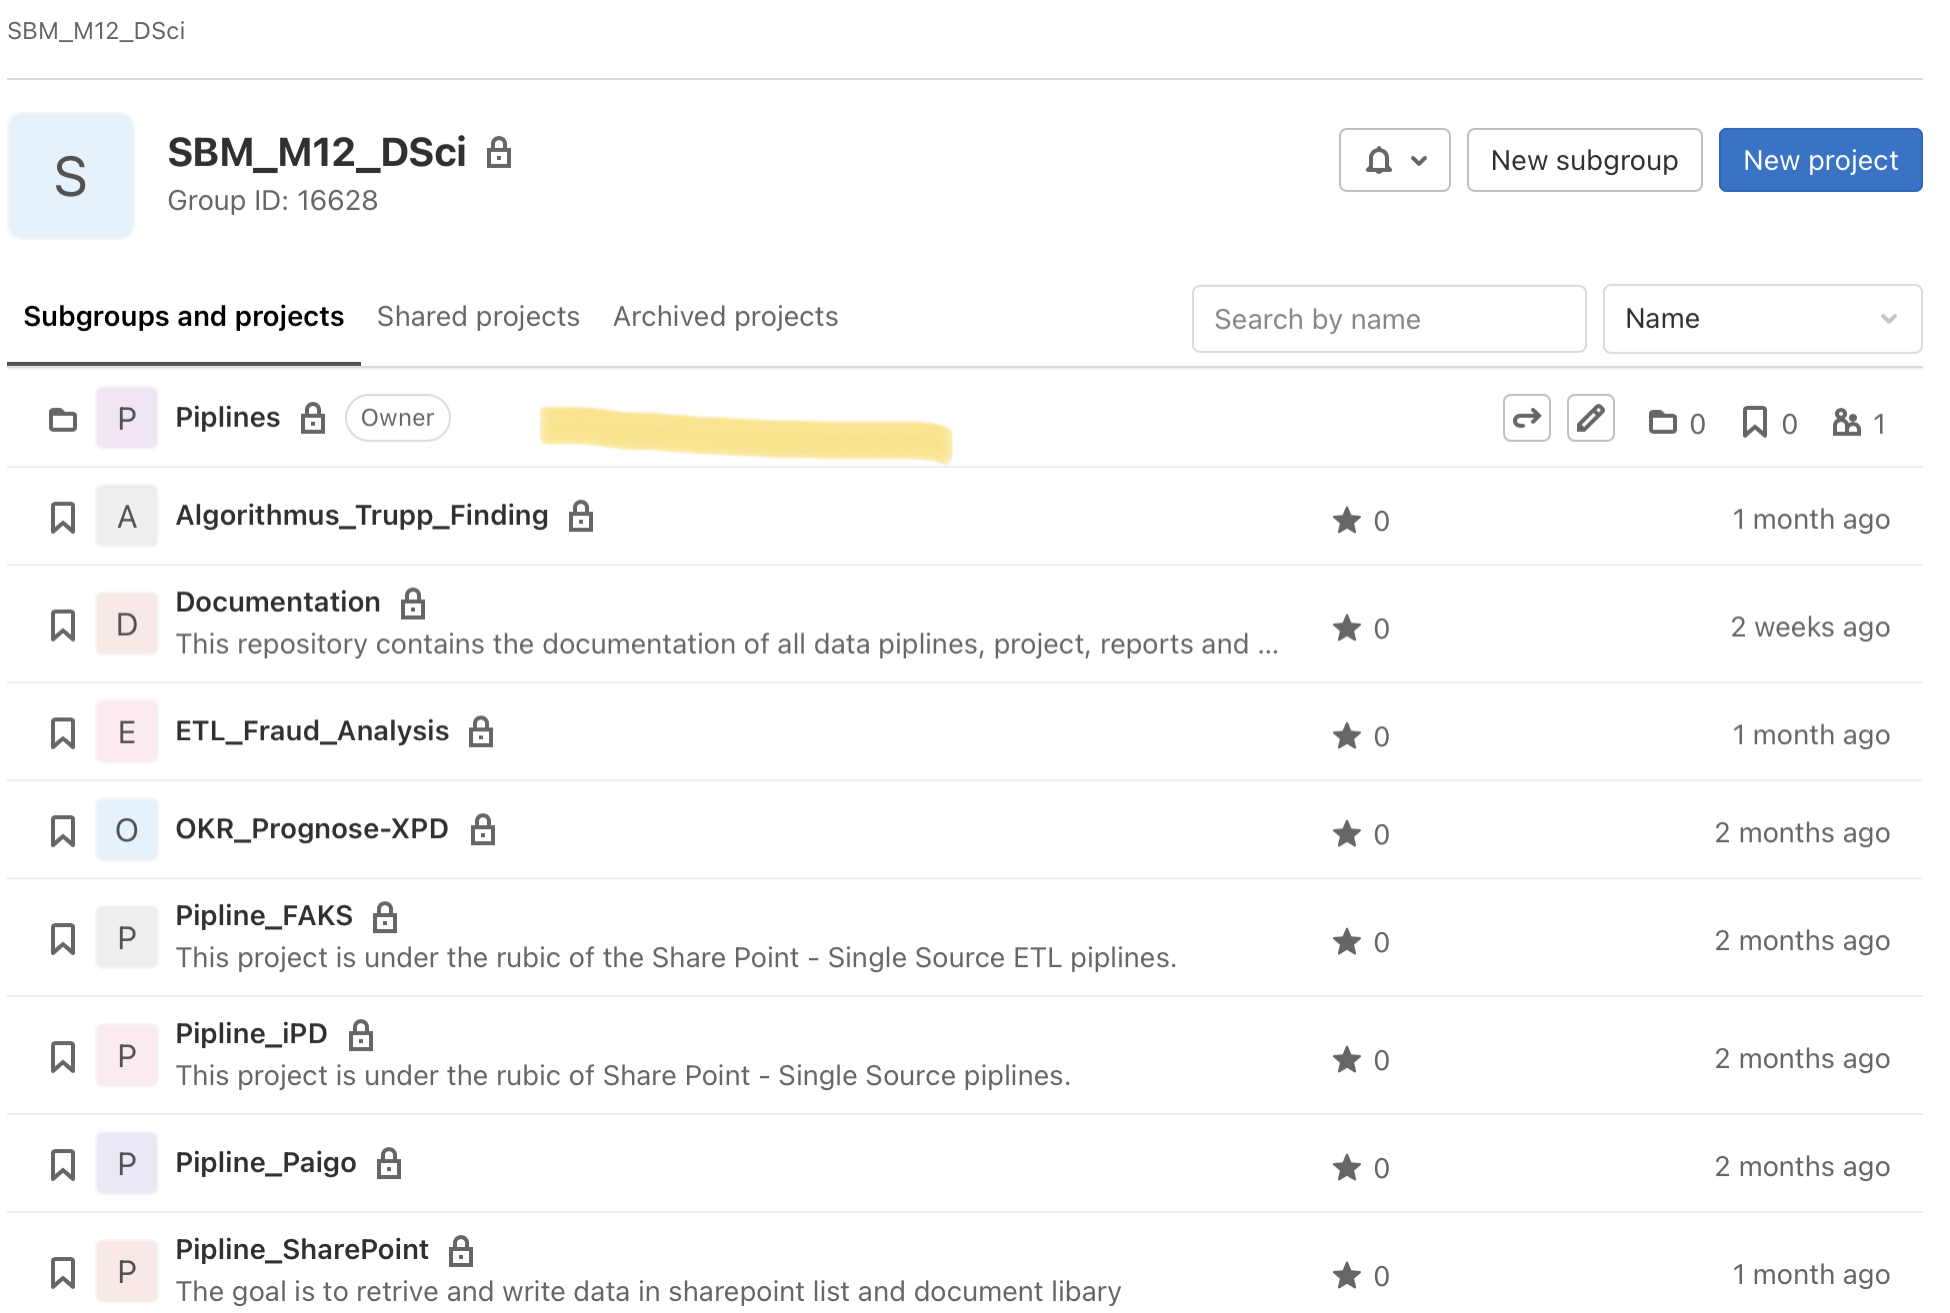
\includegraphics[width=0.7\linewidth]{attachment/chapter_5/Scc012}
\end{figure}

\subsection{Role Permissions}

\begin{figure}[H]
	\centering
	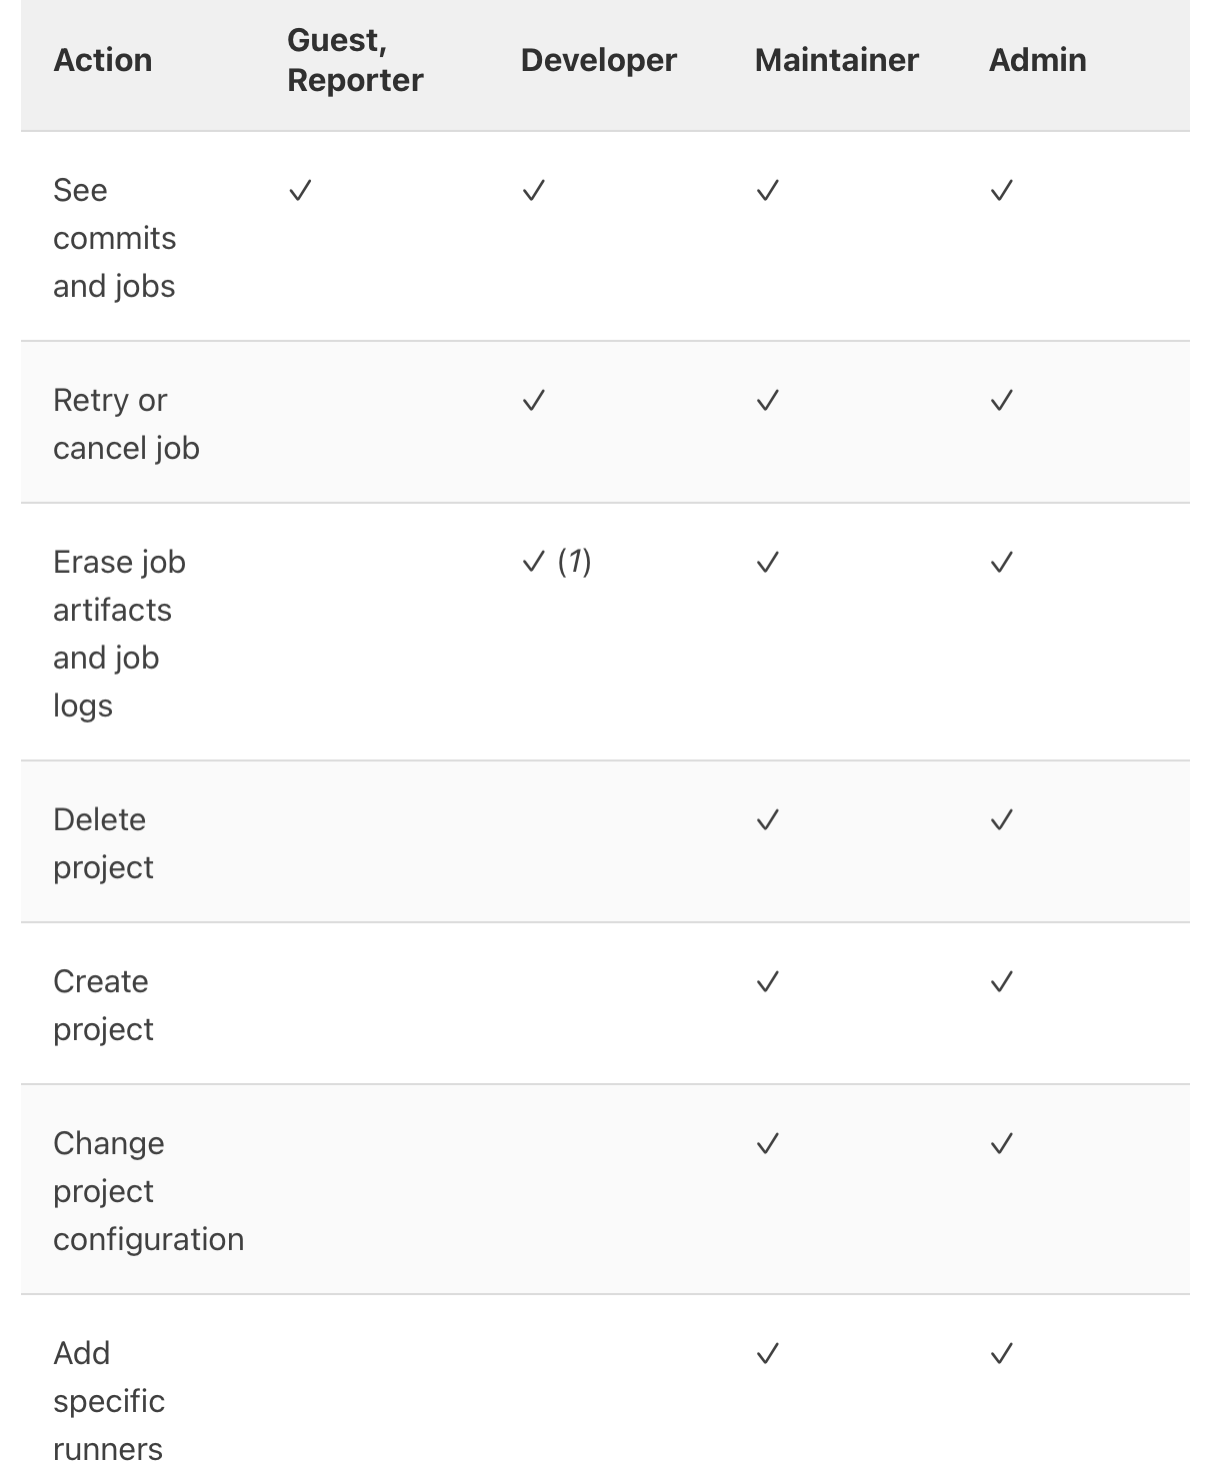
\includegraphics[width=0.7\linewidth]{attachment/chapter_5/Scc011}
\end{figure}

\subsection{Milestones}
Mehrer Issues können einem Milestone zu geordnet werden. Es gibt noch die Möglichkeit Epics zu erstellen, diese wird jedoch nicht in jedem GitLab Packet zur Verfügung gestellt.

\begin{figure}[H]
	\centering
	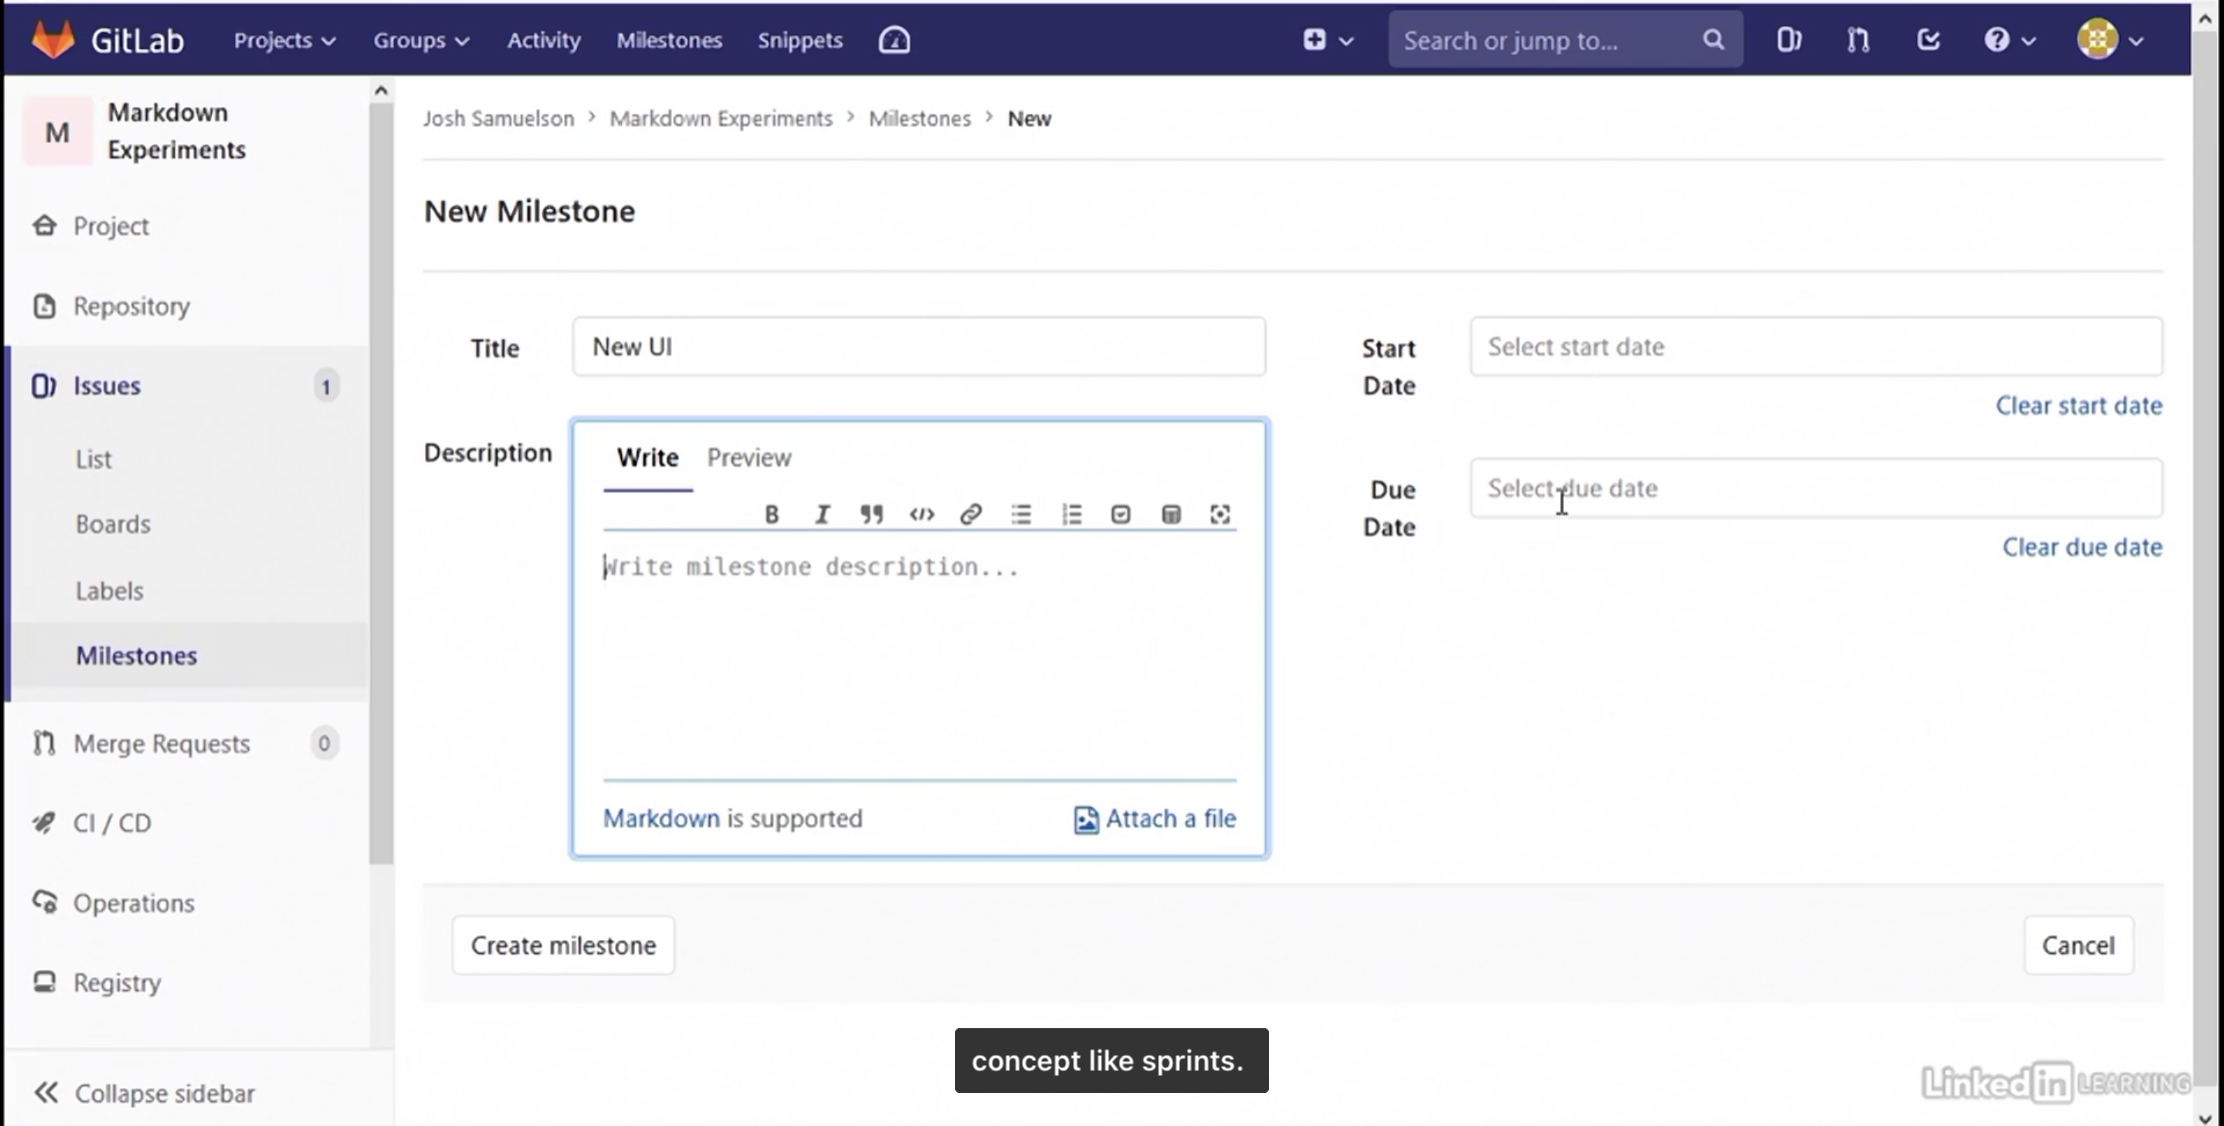
\includegraphics[width=0.7\linewidth]{attachment/chapter_5/Scc013}
\end{figure}
Bei einem Milestone wird ein Start- und Enddatum angefügt.

In der Darstellung eines Milestone wird auf der rechten Seite der Status über den Milestone angezeigt.

\begin{figure}[H]
	\centering
	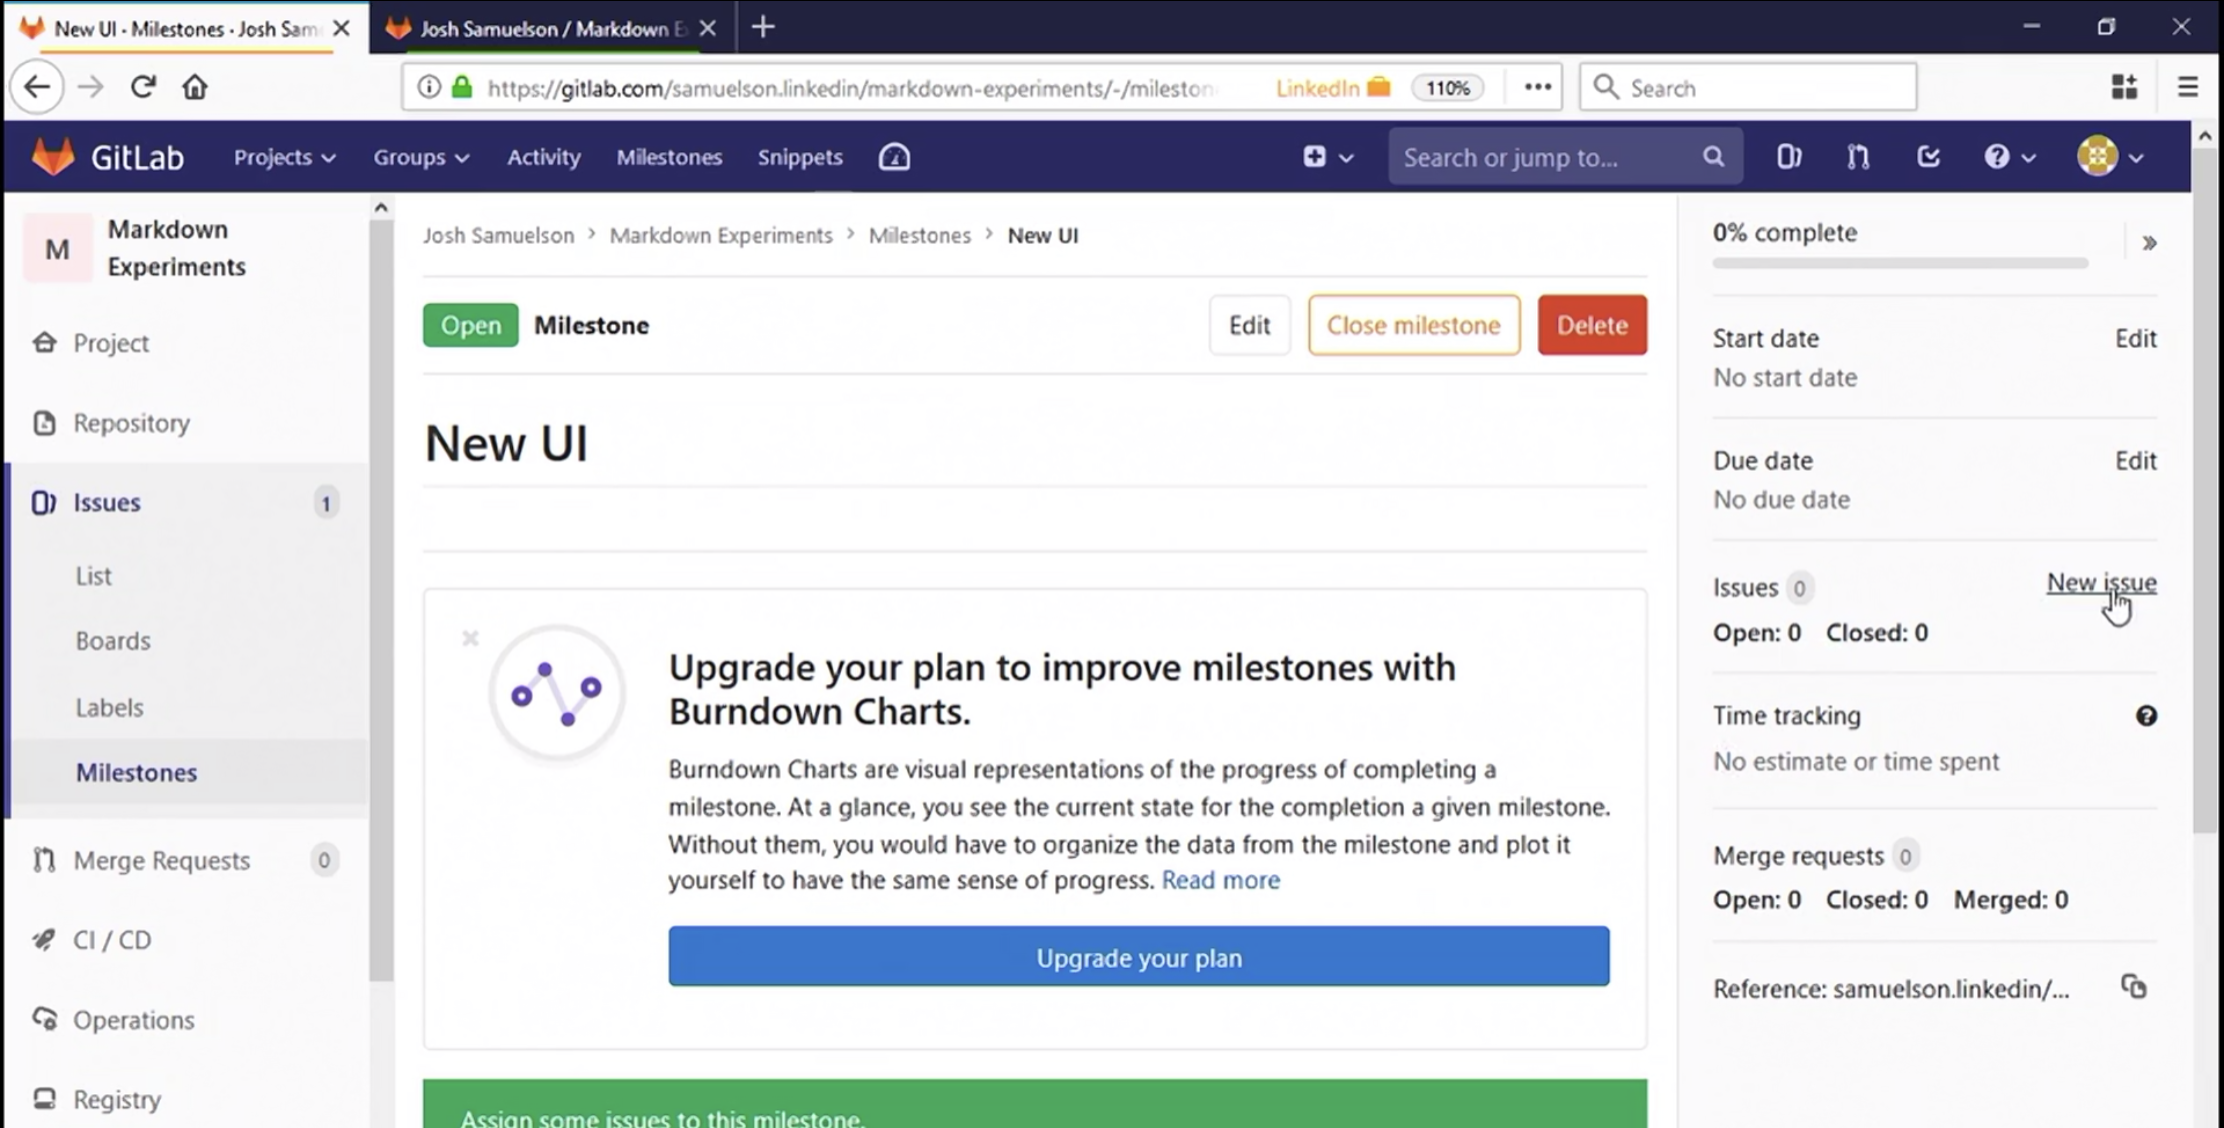
\includegraphics[width=0.7\linewidth]{attachment/chapter_5/Scc014}
	
\end{figure}

Die Funktionsweise ist, dass über jedes erstellt Issue auch eine \textit{estimed} und \textit{spend} Zeit angegeben werden kann. Hinweis: Es können mehrer Teilaufgaben zu einem Issue erstellt werden - siehe Checkboxen.

\begin{figure}[H]
	\centering
	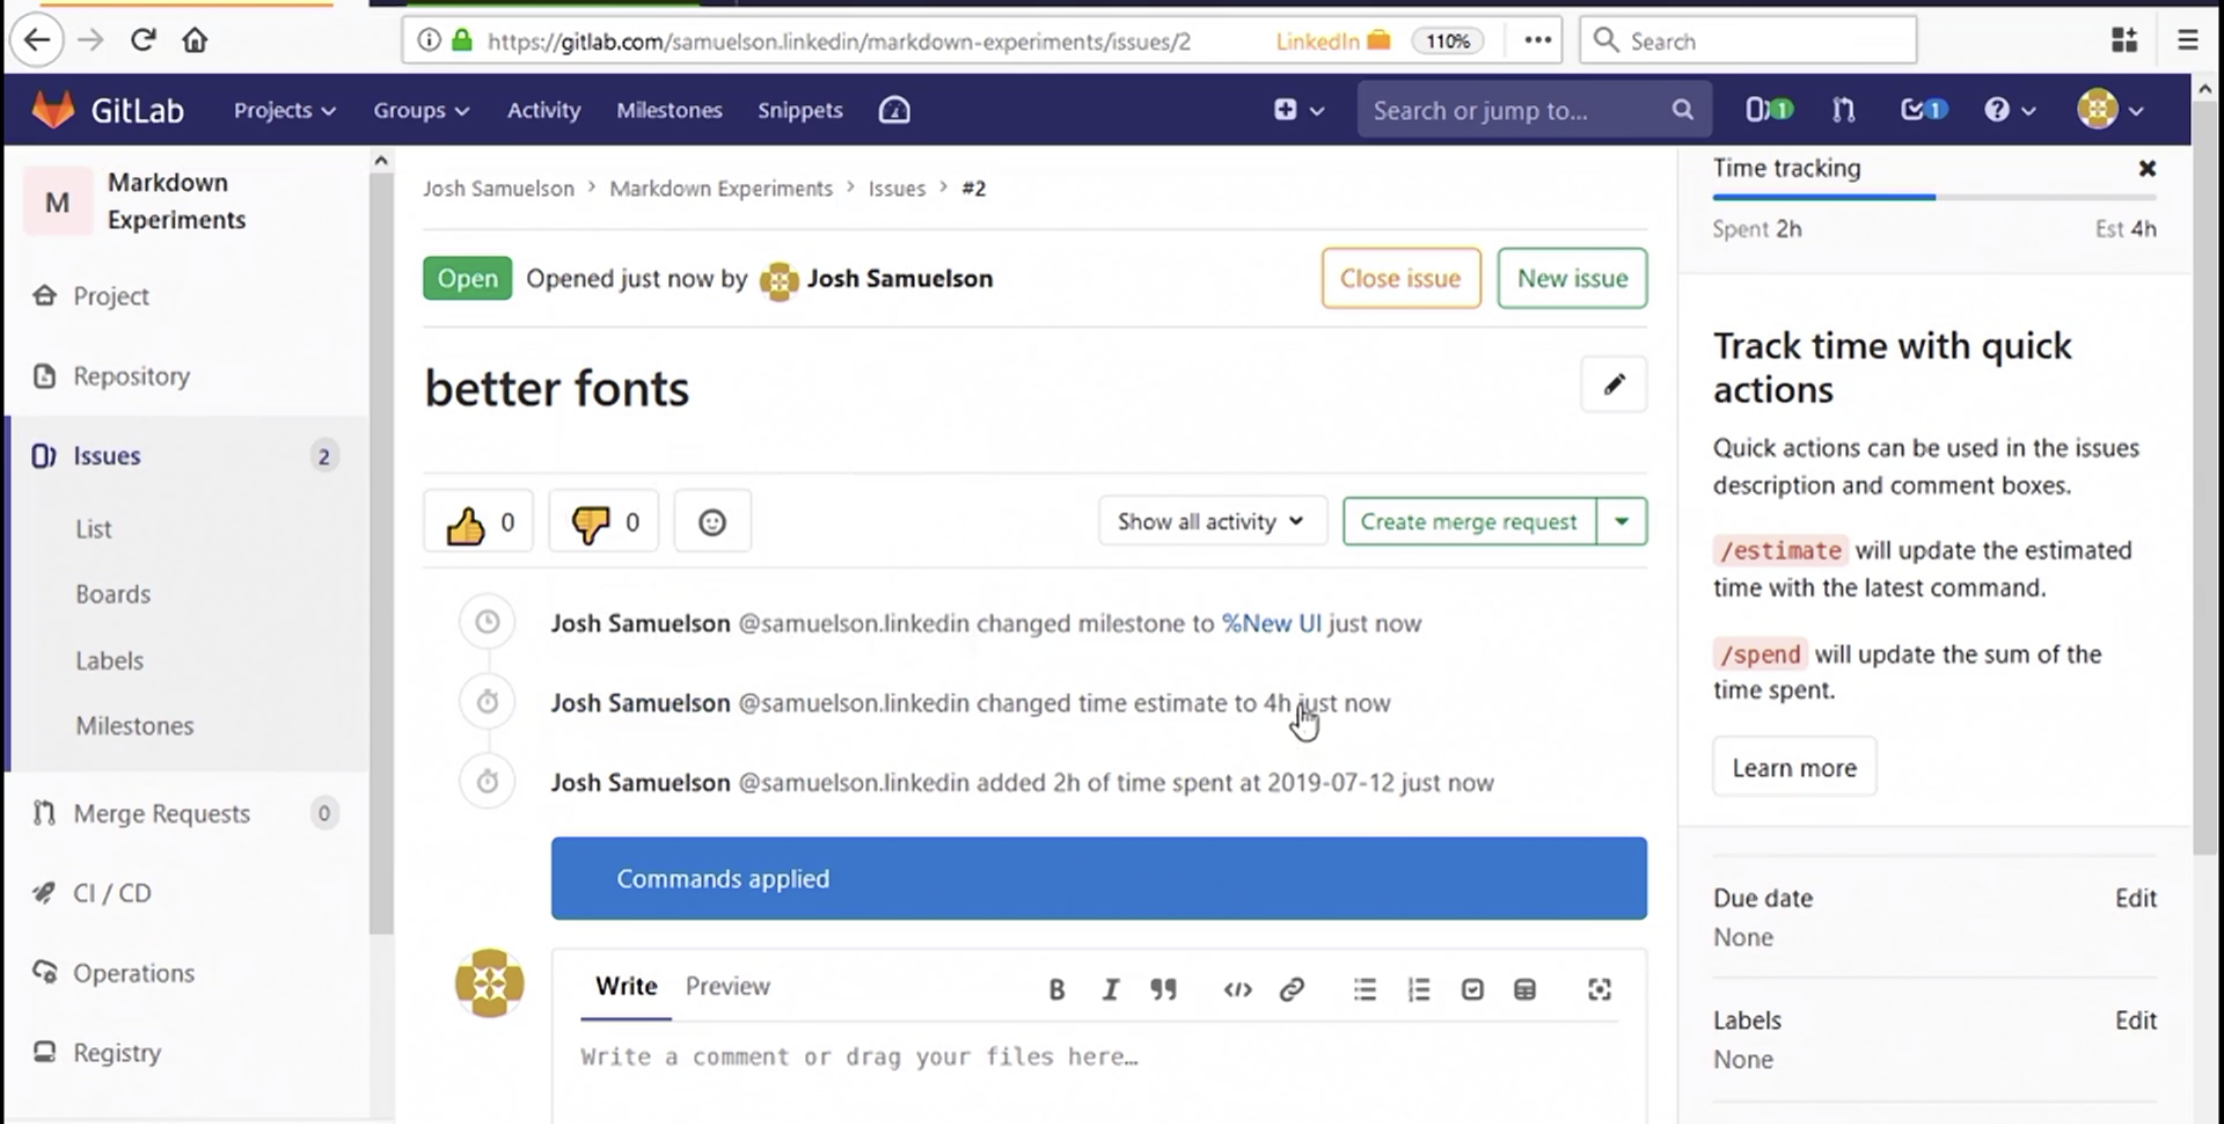
\includegraphics[width=0.7\linewidth]{attachment/chapter_5/Scc015}
\end{figure}


\section{*Vitural Enviroment Anaconda}

\section{Version Kontrolle Stategie}
Es gibt verschiedene Strategien wie in Programmierungsprojekt über \gls{g_Git} verwaltet werden können. Im Folgenden wird Bezug auf die Feature-Hotfix-Stategie von Vincent Driessen auf \href{https://nvie.com/posts/a-successful-git-branching-model/}{Successful git branching model} beschrieben wird.

\subsection{Verschiedene Branches}
\begin{itemize} 
\item master  (protected, stays)
\item develop (protected, stays, merge into master, default)
\item feature (branched from develop, merge into develop, delete after, syntax f$\_$)
\item hotfix (branched form master, merge in develop and master, delete after both merges)
\item release (optional)
\end{itemize}

\subsubsection{Master and Develop}
Es existieren zwei dauerhafte Branches im Repository. Dieses sind \textbf{master} und \textbf{develop}. Diese sind geschützt (protected). Die Einstellungen zu den beiden Branches sind,
\begin{itemize}
	\item dass nur der \textbf{Maintainer} Merger Pulls oder Push bewilligen kann.
	\item dass keine Commits gesendet werden können. Es kann nur ein Merge stattfinden.
\end{itemize}

Der \textbf{Default} Branch wird von master auf develop umgestellt. Dies hat den Hintergrund, dass Features auf Basis von Develop gebrancht werden sollen. Ebenso sollen fertige Feature Branches in Develop gemerget werden. In diesem Stadium kommt es zur Überprüfung, ob das Programm dies tut, was es tun soll. Erst dann, wird es in master gemergt, welcher als Produktion Branch fungiert.

\subsubsection{Feature and Hotfix}
\begin{itemize}
	\item In Feature branch, kann auch aus einem Issue heraus erstellt werden.
	\item Ebenso kann ein Pull-Request aus einem Issue erstellt werden.
	\item Feature werden erst in Develop eingepfelgt, wenn der Review Prozess abgeschlossen ist. \footnote{Wird über die Kommentare sich ausgetauscht, welche Änderungen noch hinzugefügt werden müssen. Der Autor kann daraufhin weitere Commits tätigen. Diese Prozess wiederholt sich, bis alle Anforderungen akzeptiert sind.}
	\item Um Komplikationen beim Merging zu verhindern, sollen features nicht auf die gleichen Dateien ändern.
	\item Es empfiehl sich, --no-ff bei Merge von Feature Branches zu verwenden. Dieser Befehlt erzeugt, ein neues Commit-Objekt am Ende. Diese verursacht mehr Komplexität, diese lässt jedoch zu, dass im Develop Branch nachzuvollziehen ist, welche Commits aus welchem Feature kommen.
	\item Hotfix ist ähnlich zu Feature. Dieser kann direkt von master gebrancht werden. Die Reparaturen werden dann in Master und Develop eingepflegt. Danach wird der Hotfix Branch gelöscht.
\end{itemize}


\subsection{Merging Optionen}
\gls{g_Git} bietet verschiedene Merging-Strategie. Einzelnen können dabei kombiniert oder gleich im der \gls{IDE} verwendet werden.
Im Folgenden werden 
\begin{itemize}
	\item Merge (fast forward)
	\item Merge Recursive
	\item Merge Squasch
	\item Merge --no --ff (no fast forward)
	\item Merge Rebase
\end{itemize}
behandelt.

\subsubsection{Merge (fast forward)}
Sei Develop Branch von Master am Punkt \textit{B} geteilt worden. Dies stellt die gemeinsame Basis für beider Branches dar.
Wurde daraufhin in Develop drei commits getätigt, und keiner in Master, kann durch in Merge ein natloser Übergang geschaffen werden.\\
\Gls{g_Git} wählt die Strategie eigenständig aus, welche am besten zur Situation passt.\\

Mit dem Merge Befehl wird Develop in Master übernommen. Dabei werden die drei Commits in Master übernommen. Liegt der Pointer bei Master wird Master wie folgt nach dem Merge dargestellt.
\begin{figure}[H]
	\centering
	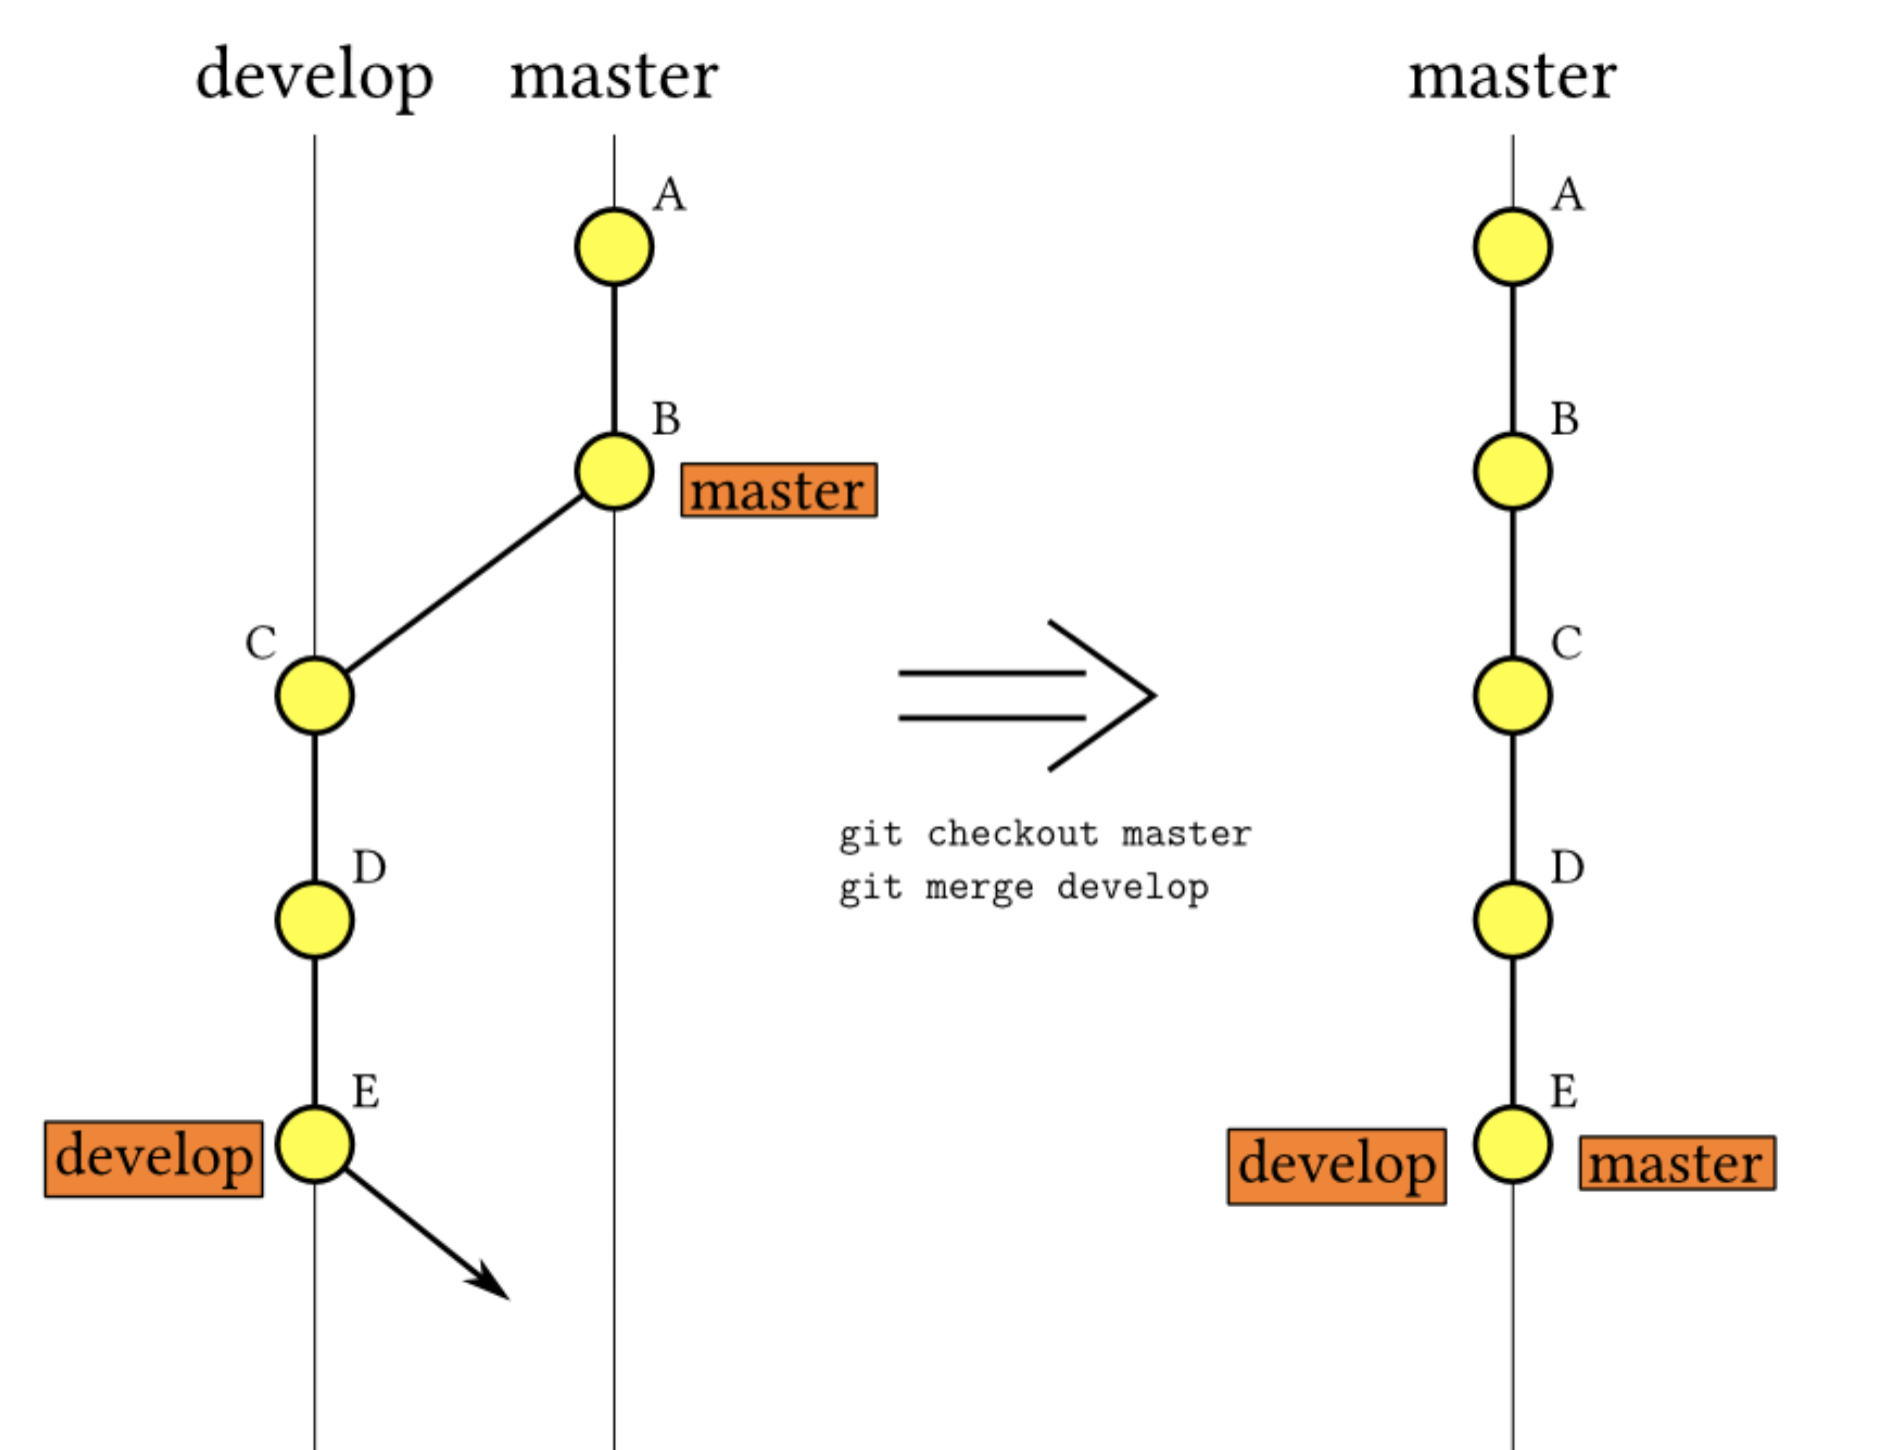
\includegraphics[width=0.7\linewidth]{attachment/chapter_5/Scc016}
\end{figure}

Das warum hinter Merge \textit{fast forward} steht, liegt daran, dass der Pointer von Master ohne ein weiteren Commit zum Ende von Develop geführt wird, ohne ein weiteren Commit auszulösen. Diese Option besteht jedoch nur, wenn in zu mergenden Branch keine Commits getätigt werden.

\subsubsection{Merge Recursive}
Feature wurde von Master vom Commit \textit{Add new file} geteilt. In Master wurden zwei Commits \textit{m1} und \textit{m2} getätigt. In Feature befinden sich zwei Commits \textit{f1} und \textit{f2}, welche nach dem Branching commetiert wurden.\\

\begin{figure}[H]
	\centering
	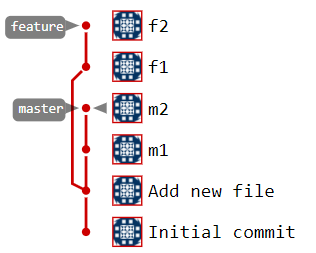
\includegraphics[width=0.7\linewidth]{attachment/chapter_5/Scc017}
	\caption{Pointer auf Master M2}
\end{figure}

\begin{figure}[H]
	\centering
	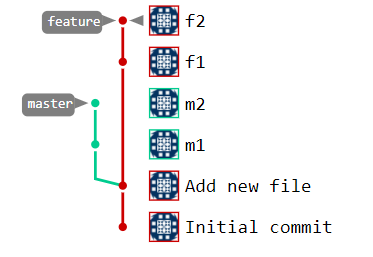
\includegraphics[width=0.7\linewidth]{attachment/chapter_5/Scc018}
	\caption{Pointer auf feature f2}
\end{figure}

Dies bedeutet, unter dem Merge-Request in Master befinden sich zwei Commits.
\begin{figure}[H]
	\centering
	
\includegraphics[width=0.7\linewidth]{attachment/chapter_5/Scc019}
\end{figure}

Wie angezeigt, wird ein zusätzlicher Commit zu Master generiert. 
\begin{figure}[H]
	\centering
	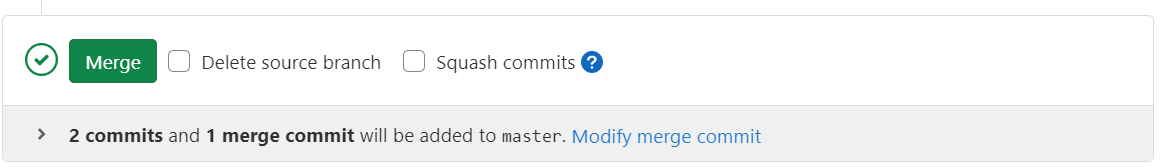
\includegraphics[width=0.7\linewidth]{attachment/chapter_5/Scc020}
\end{figure}
Die Option Feature zu löschen wird erst mal ausgelassen. Die Option Squasch commits findet sich unter \textbf{Merge Squash} wieder. Nachdem Feature unter master gemergt wurde, wird diese in dem Beispiel mit dem Commit \textit{a33fd106} festgehalten.

\begin{figure}[H]
	\centering
	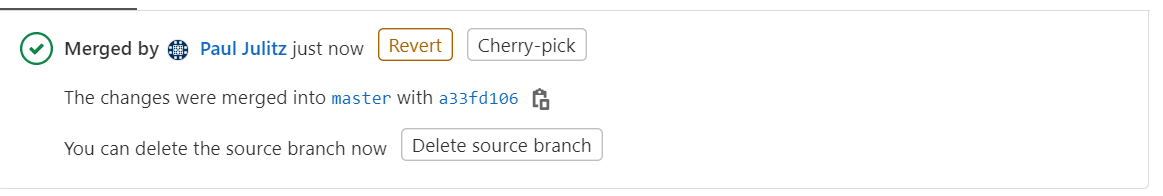
\includegraphics[width=0.7\linewidth]{attachment/chapter_5/Scc021}
\end{figure}

In Graph wird auf Master der neue Commit angezeigt, und die f2 und f1 im Feature Branch angezeigt.

\begin{figure}[H]
	\centering
	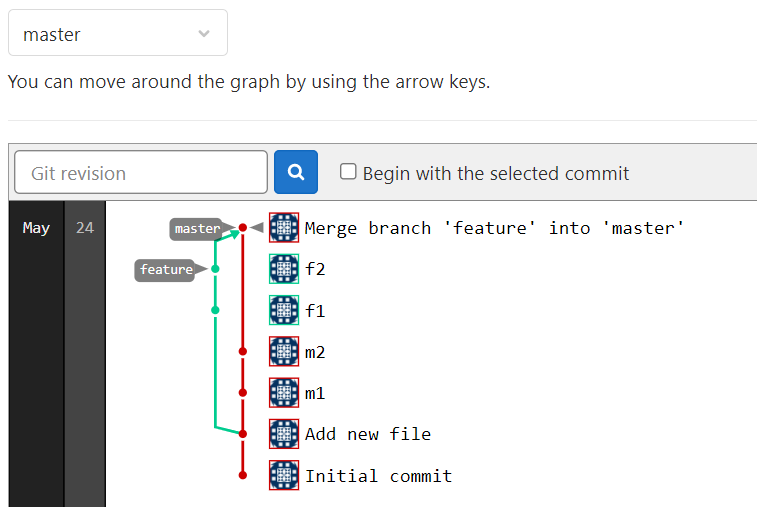
\includegraphics[width=0.7\linewidth]{attachment/chapter_5/Scc022}
	\caption{Pointer auf Master Merge Branch feature into master}
\end{figure}

\begin{figure}[H]
	\centering
	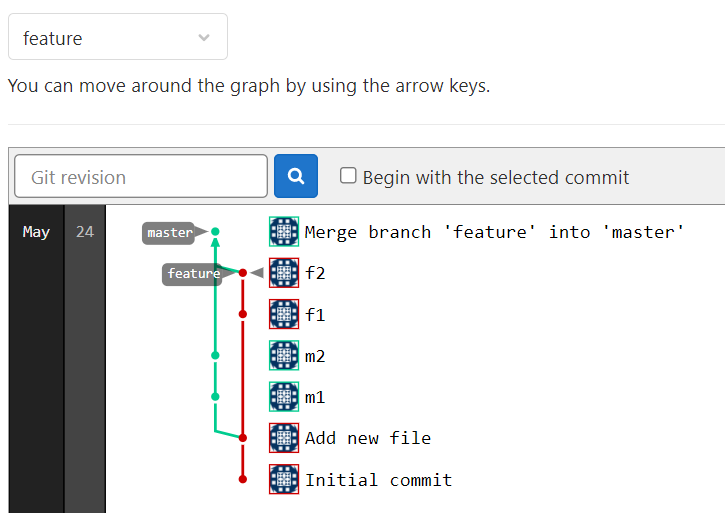
\includegraphics[width=0.7\linewidth]{attachment/chapter_5/Scc023}
	\caption{Pointer auf Feature f2}
\end{figure}

Die individuell, veränderten Dateien zweigen in Master die zugehörigen Commits an.

\begin{figure}[H]
	\centering
	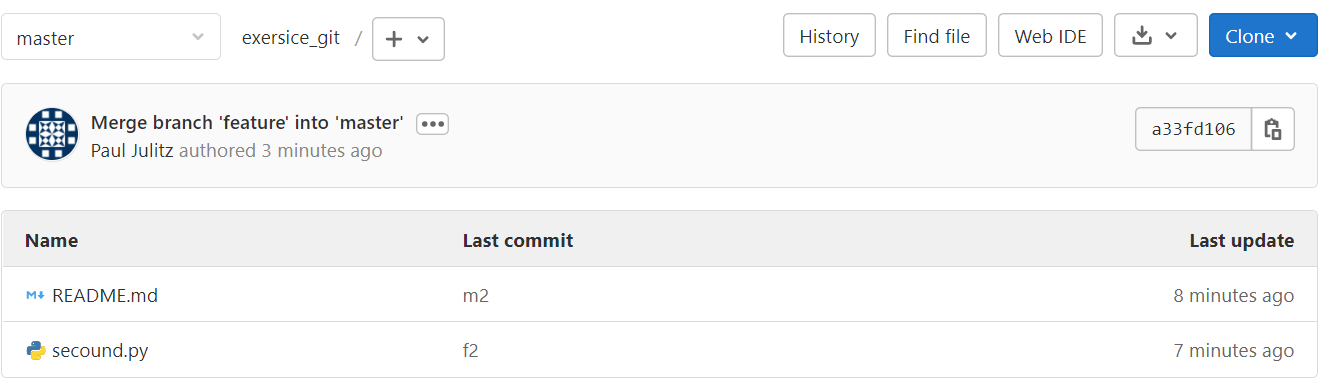
\includegraphics[width=0.7\linewidth]{attachment/chapter_5/Scc024}
\end{figure}

Die Historie zweigt alle Commits an. Mit Hinblick auf die anderen Strategien: Es wird nicht angezeigt, welcher Commit zu welchem Source Branch gehört.
\begin{figure}[H]
	\centering
	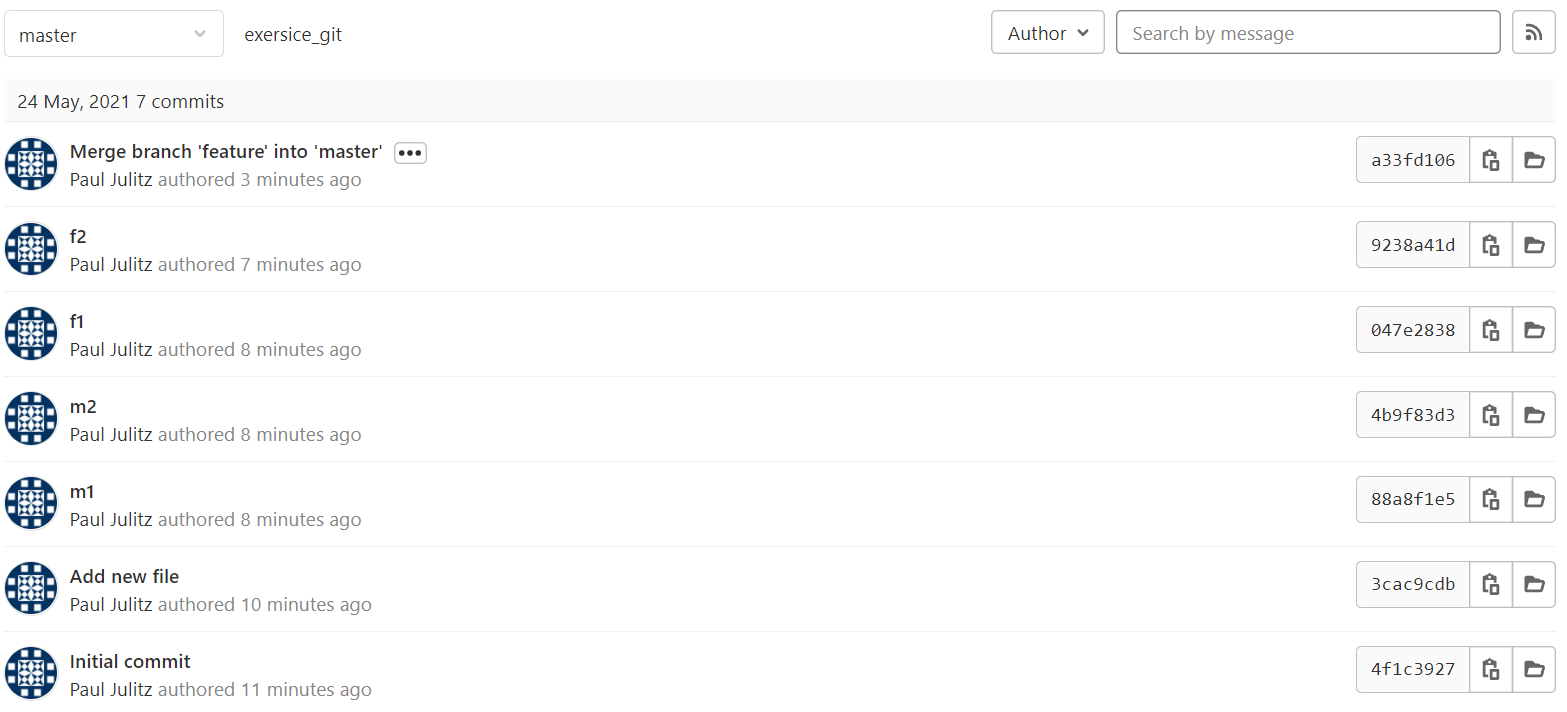
\includegraphics[width=0.7\linewidth]{attachment/chapter_5/Scc025}
\end{figure}

Wird der Feature Branch nicht gelöscht, so bleibt er weiter bestehend. Die Commits aus Master werden jedoch nicht übernommen. Weitere Commits können in Feature getätigt werden, der Commit \textit{m1} aus Master wird jedoch nicht mit übernommen. Für eine Änderung des letzten gemeinsamen Knoten wird \textbf{Rebase} verwendet.\\

Wie im Merge (fast forward) beschrieben, wählt \gls{g_Git} selbst die beste Strategie aus. In diesem Fall wählt \gls{g_Git} \textbf{Recursive Strategie} aus. Dabei wird ein Commit erstellt, welcher auf beide Branches verweist. Die Commits werden in der History unter dem Reisverschlussprinzip dargestellt. Die Strategie wird von \gls{g_Git} angewandt wenn im Sourcebranch sowie im zu commetierenden Branch Commits vorliegen.

\subsubsection{Merge Squash}
Die Option Squash 
\begin{figure}[H]
	\centering
	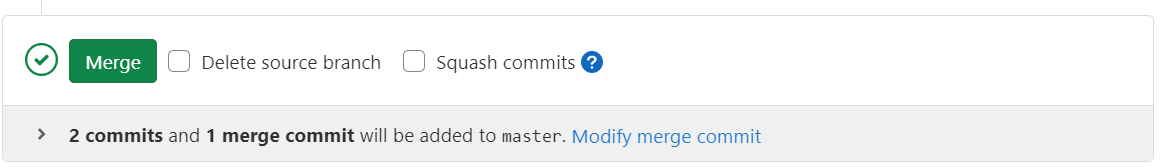
\includegraphics[width=0.7\linewidth]{attachment/chapter_5/Scc020}
\end{figure}
unter dem Merge von Feature, hätte alle Commits mit den jeweiligen Änderungen und aggregiert sie zusammengefasst. Alle Änderungen werden daher gebündetl in der Historie angezeigt.\\

Unter Feature$\_$4 wurden Commits f8 und f9 getätigt. Ebenso wurde in Master m7 hinzugefügt.
\begin{figure}[H]
	\centering
	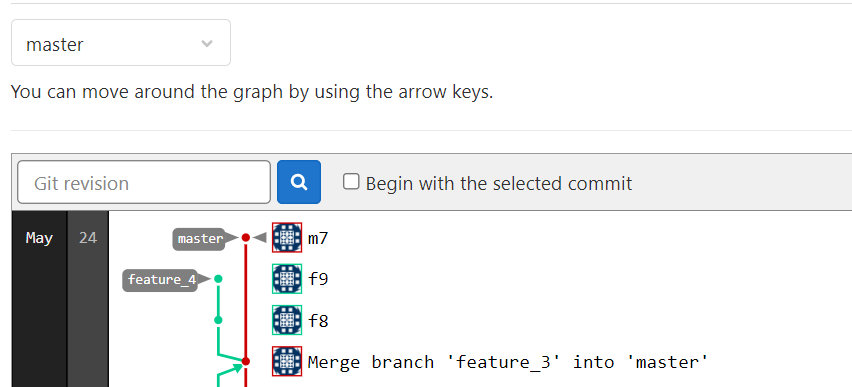
\includegraphics[width=0.7\linewidth]{attachment/chapter_5/Scc034}
\end{figure}
Wir im Merge Squash ausgewählt, wird f8 und f9 zu einem Commit zusammengefasst.
\begin{figure}[H]
	\centering
	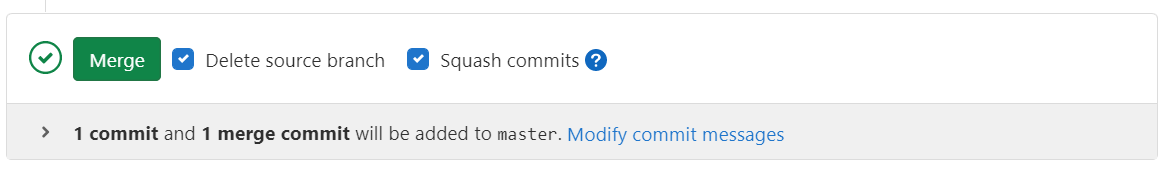
\includegraphics[width=0.7\linewidth]{attachment/chapter_5/Scc035}
\end{figure}
Weiter bleibt bestehend, dass durch die Recursive Strategy ein Commit für den Merge erstellt wird. Die Besonderheit ist, dass das Branching vom letzten Commit auf Master m7 angezeigt wird.
\begin{figure}[H]
	\centering
	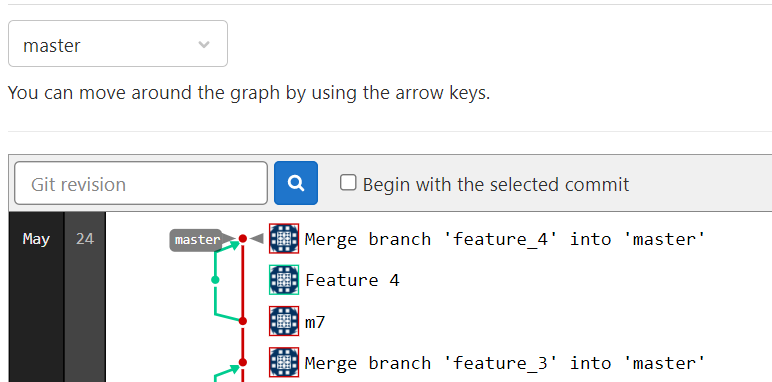
\includegraphics[width=0.7\linewidth]{attachment/chapter_5/Scc036}
\end{figure}

\subsubsection{Merge --no --ff}
Mit der Option no fastward ist ähnlich des Squash Befehl ausgeführt. Die Außnahme besteht daran, ein zusätzlicher Merge Commit getätigt wird.
    \begin{figure}[H]
    	\centering
    	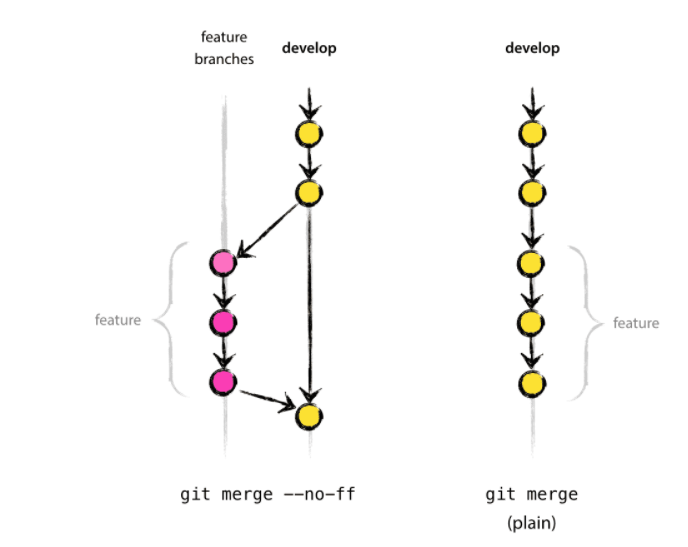
\includegraphics[width=0.7\linewidth]{attachment/chapter_5/Scc037}
    \end{figure}

\subsubsection{Rebase}
Mit der Funktion Rebase wird der gemeinsame, letzte Konten definiert. 

\begin{figure}[H]
	\centering
	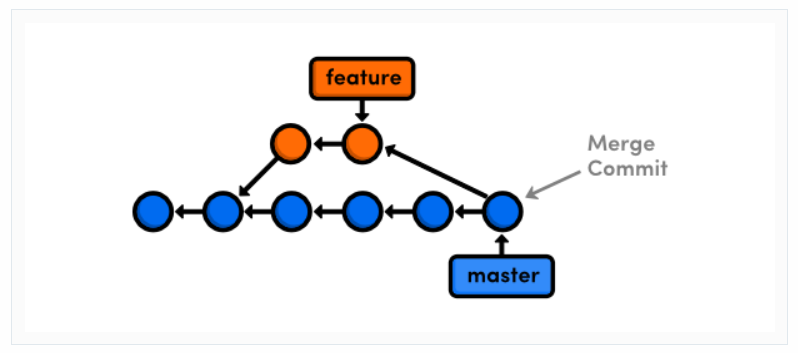
\includegraphics[width=0.7\linewidth]{attachment/chapter_5/Scc039}
\end{figure}
Mit Rebase werden alle Comits in dem Feature Branch nach dem neuen Knotenpunkt neu commetiert.

\begin{figure}[H]
	\centering
	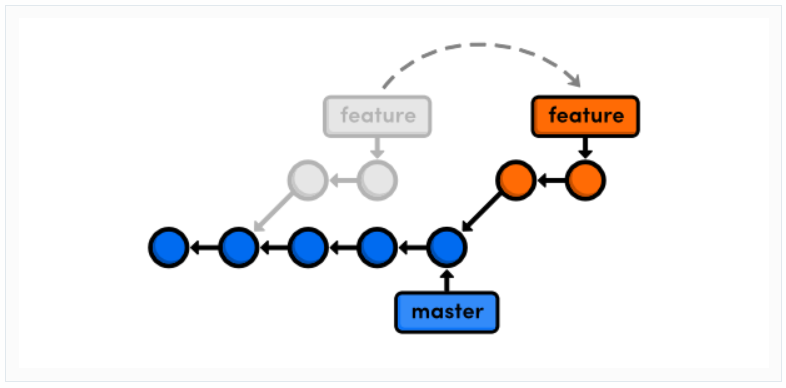
\includegraphics[width=0.7\linewidth]{attachment/chapter_5/Scc040}
\end{figure}
